\documentclass[a4paper,11pt]{article}

%\usepackage[pdftex]{graphicx}
\usepackage{amsmath}
%\usepackage[latin1]{inputenc}
%\usepackage{hyperref}
%\usepackage[T1]{fontenc}
%\usepackage[utf8]{inputenc}
%%GD Quand je mets usepackage[utf8]{inputenc} je n'arrive plus à compiler la biblio
%J'ai essayé de débuger : je n'y suis pas arrivé
\usepackage{rotating}
\usepackage{setspace}
\usepackage{lscape}
\usepackage[round]{natbib}
\usepackage{multirow}
\usepackage{rotating}
\usepackage{vmargin}
\usepackage{epstopdf}
\usepackage{hyperref}
\usepackage{float}
\usepackage{caption}
\usepackage[tableposition=top]{caption}
\usepackage{amsfonts}
\usepackage{bbold}
\usepackage{bbm}
\usepackage[flushleft]{threeparttable}
%\usepackage{bbold}
%\usepackage[T1]{fontenc}
% JH : impossible de compiler avec le package bbold, remplacé par amsfonts
% LP : impossible de compiler avec le package bbold, remplacé par bbm
\usepackage{upgreek}
\usepackage{comment}
\includecomment{commentGD}
\usepackage[draft]{todonotes}
%\usepackage[disable]{todonotes}
%%GDPour cacher les notes, \usepackage[disable]{todonotes}


%\usepackage[nolists, figuresfirst]{endfloat}
%\usepackage{sidefloat}

\setlength{\abovecaptionskip}{-8pt}

%\usepackage[usenames]{color}
%\definecolor{grey}{rgb}{0.35,0.35,0.35}
%\definecolor{webdarkblue}{rgb}{0,0,0.4}
%\definecolor{orange}{rgb}{0.7,0.2,0.05}


%\usepackage[pdfcreator={PDFLaTeX}, pdfproducer={PDFLaTeX}, pdfstartview=FitH, pdfpagemode=UseOutlines, pagebackref=false, colorlinks={true},
%citecolor={webdarkblue}, linkcolor={webdarkblue},
%urlcolor={webdarkblue}]{hyperref}



%\addtolength{\oddsidemargin}{-0.4in}
%\addtolength{\evensidemargin}{-0.4in}
%\addtolength{\textwidth}{0.8in} \addtolength{\topmargin}{-0.85in}
%\addtolength{\textheight}{1.7in}
\renewcommand{\baselinestretch}{1.2}

\newcommand\cites[1]{\citeauthor{#1}'s\ (\citeyear{#1})}

\newcommand\citeh[1]{\citeauthor{#1}'\ (\citeyear{#1})}

\setmarginsrb{3cm}{2cm}{3cm}{2cm}{0,5cm}{0,5cm}{0,3cm}{0,5cm}



% commands

\newcommand{\bi}{\begin{itemize}}
\newcommand{\ei}{\end{itemize}}
\newcommand{\be}{\begin{enumerate}}
\newcommand{\ee}{\end{enumerate}}
\newcommand{\bd}{\begin{description}}
\newcommand{\ed}{\end{description}}
\newcommand{\beqa}{\begin{eqnarray}}
\newcommand{\eeqa}{\end{eqnarray}}
\newcommand{\beq}{\begin{equation}}
\newcommand{\eeq}{\end{equation}}
\newcommand{\bs}{\bigskip}
\newcommand{\A}{$^a$}
\newcommand{\B}{$^b$}
\newcommand{\C}{$^c$}

\begin{document}




\title{\textsc{International Transport costs:\\New Findings from modeling additive costs}\thanks{We are grateful to S\'{e}bastien Jean, Vincent Vicard, and participants at ETSG 17\textsuperscript{th} meetings in Helsinki, DEGIT XXII in Paris School of Economics, and participants at seminars of the University of California-Irvine, the Universities of Paris-Dauphine Paris-I and Nancy for very useful discussions.
Finally, any remaining errors are ours.
This paper features an online appendix containing additional results and available on the authors' websites.}}

\author{Guillaume \textsc{Daudin}\thanks{%
Universit\'{e} Paris-Dauphine, Université PSL, IRD, LEDa, UMR 225, DIAL, 75016 PARIS, FRANCE \newline
Sciences Po, Observatoire Fran\c{c}ais des Conjonctures \'{E}conomiques (OFCE), 75014 PARIS, FRANCE \newline
; email: \url{guillaume.daudin@dauphine.fr}}  \qquad J\'{e}r\^{o}me \textsc{H\'{e}ricourt} \thanks{Universit\'{e} de Lille - LEM-CNRS UMR 9221, France \& CEPII, France; email: \url{jerome.hericourt@univ-lille.fr}}\qquad Lise \textsc{Patureau}\thanks{Corresponding author.
Universit\'{e} Paris-Dauphine, Université PSL, LEDa, 75016 PARIS, FRANCE;  email: \url{lise.patureau@dauphine.fr} } }


\date{June 2018}
 \maketitle
\bigskip

\begin{abstract}
This paper investigates the role of additive costs in international transport costs, using information contained in a US imports flows database over 1974-2013.
We find that the additive component of transport costs is sizable, representing between one third and one half of overall transport costs.
Further, in the same spirit as \cite{hummels2007}, we identify the respective roles of the reduction in ``pure'' transport costs and changes in trade composition effects in the downward trend of international transport costs. In contrast to \cite{hummels2007}, we find that trade composition effects do not matter much and, when they do, they tend to amplify (rather than reduce) the decrease in pure transport costs.
Importantly, this difference of results can be attributed to the new way of modeling the per-unit (additive) component of transport costs we offer.
In both aspects, our results point to the importance of the additive component in accounting for international transport costs.
\end{abstract}


\thispagestyle{empty} \pagestyle{plain} \setcounter{page}{1}

\bigskip


\noindent \emph{JEL classification}: F14, N70, R40 \\
\noindent \emph{Keywords}: Transport costs estimates, non-linear econometrics, period 1974-2013, additive costs, trade composition effects

{\normalsize \vspace{0cm} }

{\normalsize \titlepage }

{\normalsize \newpage }

%\begin{spacing}{1.5}

\section{Introduction \label{sec:Intro}}

Trade costs are central to international economic analysis.
In particular, they are known to be a major obstacle to international economic integration and international trade flows.
Based on panel data, \citet{novy13} finds  that U.S.
trade costs with major trading partners declined on average by about 40 percent between 1970 and 2000.
Trade costs declined faster for more developed countries (\citealp{arvis2016trade}).
Still, several papers (mostly based on empirical estimates of the gravity equation) have shown that trade costs remain a major obstacle to trade (\citealp{Head_Mayer04} or \citealp{Disdier_Head08}, to name a few).
Using data over 1989-2000, \citet{anderson_wincoop_jel} thus estimate that average international trade costs represent a 74\% markup over production costs for industrialized countries.


Defined as the costs associated with the exchange of goods across national borders, trade costs are usually split between transaction costs (information costs, contract enforcement costs, costs associated with the use of different currencies...), policy costs (tariffs  and non-tariff costs), time costs (time to ship goods) and transport costs \emph{per se}.
In this vein, \citet{anderson_wincoop_jel} obtain that around 30\% of international trade costs are attributable to transport costs.
Equivalently, international transportation costs represent a 21\% markup over production costs.
Further, the sizable elasticity of trade with respect to freight costs obtained by \cite{Behar_Venables} (around -3) testifies to the impact of transport costs on trade flows.
If much of trade policy barriers have been removed over the second half of the twentieth century, this suggests that the transport costs component remains large and deserves attention.
International transport costs accordingly stand at the heart of the paper.\smallskip

This focus is shared with part of the international trade literature that studies the patterns of transport costs over time, such as \cite{hummels2007} and \cite{Behar_Venables}.
Many argue that transport costs have substantially decreased with technological advance in transportation (\citealp{levinson2016box}), infrastructure development and new communication technologies (\citealp{Lafourcade_Thisse}).
There is no consensus thought.
Distance as an incompressible cost is still a very important determinant of trade flows (\citealp{Disdier_Head08}); further, progress in transportation techniques (that reduces the constant-dollar cost of transport) should be compared with technical progress in production (that reduces the constant-dollar cost of production) to get a clear picture of the evolution of the transport costs burden.
In accordance with this view, \cite{hummels2007} points out that transport costs in proportion of export prices have declined more slowly than the common wisdom assumes.\smallskip

According to \cite{hummels2007}, this lower-than-expected decline of transport costs is partly explained by trade composition effects (i.e., changes over time in the baskets of imported goods and/or the origin countries).
Based on US imports over 1974-2004, he finds that total transport costs have decreased in both air and maritime shipment, but less so than ``pure'' transport costs (i.e., \textit{ceteris paribus} for given goods, mode, and trade routes) because trade composition effects have partly offset the pure transport costs decrease, thereby attenuating the overall transport costs downward trend.\footnote{Throughout the paper, we refer to ``pure'' or ``per se'' transport costs changes as the changes over time in the transport costs for a given product/country partner, ie excluding trade composition effects.} In this paper, we dig deeper into this issue.
As a major contribution, and in contrast to \cite{hummels2007}, we find that trade composition effects play a minor role in accounting for the trend patterns of transport costs.
Rather, the evolution of transport costs ``per se'' constitutes the main driving force behind the overall transport costs decrease, in particular for air transport.
In maritime shipment, trade composition effects matter more, but they amplify (rather than offset) the reduction in pure transport costs.
In this respect, we find that pure transport costs declined even less since the 1970s than argued by \cite{hummels2007}.\medskip

Proving this point drives us to provide a careful modelling of transport costs.
Following \citet{samuelson1954}, standard models of international trade have usually modeled trade costs as an \emph{ad-valorem} tax equivalent (ie, as a constant percentage of the producer price per unit traded, part of the ``iceberg cost'' hypothesis).\footnote{Strictly speaking, the ``iceberg cost'' includes both the ad-valorem dimension of trade cost and the fact that these costs are paid in terms of the good that is traded.
As this last element is irrelevant in our case, we use the terms ``iceberg'' and ``ad-valorem'' interchangeably, as it is commonly done in the literature.} However, a recent strand of the literature points out to the existence of an additive component, that is, a cost per unit traded (see, among others, \citealp{Irrazabal_2015} or \citealp{martin2012}).
Based on US sectoral data, our own estimates also bring out the importance of additive costs in international transport costs.
We obtain this by providing an empirical decomposition of the structure of transport costs over time, in which we explicitly distinguish between ad-valorem and additive costs.
To do so, we exploit information contained in the Census Bureau's database of US imports flows over 1974-2013.
This database contains a measure of international transport costs as the difference between the import and the export prices, on a year-product-partner country basis.
This database is the same as \cite{hummels2007}, extended over more recent years (2005-2013).
\smallskip

Our results may be summarized in two main new findings.
First, additive transport costs are quantitatively sizable.
On average over 1974-2013, the additive cost is estimated to be 1.8\% and 2.9\% of the export price in air and vessel transport respectively.
This is slightly lower than our estimates for the ad-valorem component (2.5\% and 3.2\% for air/vessel respectively on average over the period).
Put it differently, additive costs represent between one third and almost one half of the overall transport costs.
%\textbf{GD Pourquoi est-ce qu'en faisant le calcul je trouve 33\% et 47,5\% ?}
To the best of our knowledge, our paper is the first to provide such an extensive quantitative measure of both ad-valorem and additive costs in total transport costs.
This represents a valuable insight for calibrating related international trade or business cycle models.
We also provide an empirical assessment of what standard international trade models lose by skipping additive transport costs.
Quantitatively, the omission of the additive term leads to overestimate the ad-valorem component by roughly a factor~2.

Second, we find that the main source of the downward trend in overall transport costs -by roughly 50\% in air shipping and 60\% in vessel shipping over 1974-2013, comes mainly from the reduction of transport cost ``per se''.
Trade composition effects only have a limited influence, and when they matter (in maritime transport), composition effects amplify the reduction of pure transport costs.
Otherwise stated, pure transport costs have declined less than observed costs.
This stands in contrast to the conclusion obtained by \cite{hummels2007} on the same database (until 2004).
Our result thus deepens the paradox of the less-than-expected decline of transport costs.
Importantly, we show that the difference of results can be attributed to the new way of modeling of the additive component we offer.
Allowing the share of additive costs to vary across time, products and country partners (rather than being constant as in \citealp{hummels2007}), turns out to be key in the decomposition of underlying sources of the decrease of overall transport costs observed over the period.
\smallskip

In both aspects, our results point the importance of the additive component in accounting for international transport costs.
In this respect, it contributes to the literature that challenges the dominant role of iceberg costs in international trade (even in the case of ice transport, see \citealp{bosker2018ice}).
As shown by \cite{alchian}, the relative price of two varieties of some good will depend on the level of additive trade costs.
In this context, the relative demand for more expensive/higher quality product goods increases with trade costs (``shipping the good apples out'').
This is consistent with the findings by \citet{hummels_skiba}, who estimate the elasticity of freight rates with respect to price to be well below unity.
Also, their estimates imply that doubling freight costs increases average free alongside (fas) export prices by 80 to 141 percent, consistent with high quality goods being sold in markets with high freight costs.
Recent empirical studies based on micro-level data also provide a strong empirical support to the role of additive costs (i.e., cost per unit exported) in international trade costs.
Based on a firm-product-level database of French exporters, \citet{martin2012} finds that firms charge higher unit values for exports to more remote countries, supporting the importance of additive costs.
Using transaction-level trade data from Colombia, \cite{Lashkaripour-2017b} estimates that the transport cost elasticity varies greatly across industries, with a value of 0.8 for the average industry, in contrast with the iceberg specification.\footnote{Beyond the positive aspect, several recent papers also point out the normative implications of additive trade costs.
\citet{sorensen2014} extends \citet{melitz}'s seminal model of international trade by including additive trade costs, in addition to the ad-valorem component.
A key analytical result is that the welfare gain from a reduction in trade barriers is higher for a decrease in additive costs than a decrease in ad-valorem costs, due to the alteration of relative prices in a heterogeneous-firms trade framework.
This is confirmed by \cite{Irrazabal_2015}.
While these results suggest that important welfare gains can be achieved by reducing additive trade costs, not much progress has been done in quantifying such gains.
One potential reason is the lack of an empirical characterization of the additive component of trade costs (the one exception being \citealp{Irrazabal_2015}).
One contribution of the paper is to fill this gap.}

Closely related to our paper is the work by \citet{Irrazabal_2015}, which develop a structural framework for inferring relative additive trade costs from firm-level trade data.
Implementing their methodology on Norwegian firm-level export data for the year 2004, they find that, for the median shipment, additive costs (in Norwegian crowns) amount to 6\% of the export price multiplied by the ad-valorem cost (also expressed in Norwegian crowns).
Our results share in common with \citet{Irrazabal_2015} the important role of the additive component of international trade costs.
Yet, our paper complements their findings in two main respects.
First, while our study covers a narrower set of trade costs focused on transport costs, their data and their empirical approach only allows the identification of the ratio of the additive cost to the export price multiplied by the ad-valorem cost ; by contrast, our estimation strategy enables us to uncover separately both values of the ad-valorem and the additive costs.
From this, we can rebuilt the ratio in similar terms to them, thereby gaining in generality in this respect.
While \citet{Irrazabal_2015} obtain that, for an export price multiplied by the ad-valorem cost of 100 USD, 6 USD are paid in additive trade costs, our own results point to a value paid in additive transport costs of 2.8 USD for maritime shipping and 1.5 USD for air transport for 2004.
This comparison of results suggests that between a third and a half of the additive trade costs are attributable to the transport sector (depending on the transport mode).
Second, we exploit exhaustive information about the imports flows of the US over a large time span from 1974 to 2013.
In this respect, our results deliver a broader view of the magnitude of additive costs in international trade over time.
In particular, we show that the modeling of additive costs is of critical importance in determining the underlying sources of the trends patterns of international transport costs observed since 1974.\footnote{On top of the previously cited papers about additive costs, our paper also relates to \citet{Kropf-Saure-JIE-2016}, which estimate the size and shape of per-shipment costs bases on Swiss data, and to \citet{Alessandria-et-al-AER-2010} or \citet{Hornok-et-al-JIE-2015, Hornok-et-al-RES-2015}, which point out the role of per-shipment costs (among which, administrative costs) in generating some ``lumpiness'' in international trade transactions.} \smallskip

%\textbf{enleve ancienne footnote plus haut qui reprenait cette difference, a mettre en footnote ici? en commentaire en dessous}
%However, given their database and their empirical approach, \citet{Irrazabal_2015} can only identify the ratio of the additive to the ad-valorem cost ($\frac{t_{ik}}{\tau_{ik}}$ in our terminology), that they interpret by expressing it in terms of the median export price by country-product ($\bar{\widetilde{p}}_{ik}$).
By contrast, our estimation strategy enables us to uncover both values of the ad-valorem and the additive costs $\tau_{ik}$ and $t_{ik}$ separately, in terms of the country-product export price $\widetilde{p}_{ik}$.

The paper is built as follows.
First, we estimate the values of international transport costs annually throughout the period 1974-2013 by transport mode, explicitly distinguishing between the additive and the ad-valorem components.
 Section \ref{sec:data_method} thus reports the mean values of the transport costs estimated over the period (by transport mode).
Relying on these estimation results, we then provide a decomposition of the transport costs trend patterns, between what comes from changes in the trade composition (by product and/or partner country), and what is attributable to changes in transport costs ``per se''.
Section \ref{sec:results_trends} is devoted to this analysis, while section \ref{sec:robustness} checks the robustness of our results to the separability assumption and the weighting scheme.
Section \ref{sec:conclu} concludes.


\section{Estimating international transport costs\label{sec:data_method}}

\subsection{Data}

Our analysis of transportation costs consists in exploiting the difference between commodity-level export and import prices, as in \cite{hummels2007}.
The database we use to construct our measure of transport costs comes from US annual "Imports of Merchandise" provided by the Census bureau, spanning from 1974 to 2013.
Details on the database are provided in Appendix \ref{app:data}.
We first use customs values, quantities and freight costs to recover free-alongside (fas) and cost-insurance-fret (cif) prices, by good, country of origin and transportation mode.\footnote{The related literature commonly refers to the fob price rather than the fas price.
The fas price (for ``Free Alongside Ship'') means that the seller must transport the goods all the way to the dock, close enough to be reached by the crane of the ship it will be transported in.
It is also the seller's responsibility to clear the goods for export.
The fob price (for ``Free on Board'') means that the seller is obligated to bring the goods all the way to the port, clear the goods for export, and see that they are loaded onto the ship nominated by the buyer.
Once the goods clear the railing of the vessel the buyer assumes the risk.
Note that this term is used exclusively for maritime and inland waterway transport.
While both terms are closely related, the US Foreign Trade Statistics reports fas prices.} More precisely, the (unit) fas price is computed as the total ``customs value'' in the US trade statistics divided by the shipping weight; in other words, it is the price for one kg of the good net of transportation costs.
The cif price is then computed as the sum of the customs value and freight charges, once again divided by the shipping weight.
Our dependant variable is finally computed as the ratio of the cif price divided by the fas price.
By construction higher than 1, the variable provides a measure of transport costs as a proportion of the good's price, an \emph{ad-valorem} equivalent.
This is a quite standard and widespread strategy, as emphasized by \citet{anderson_wincoop_jel}.

Obviously, this dataset has limitations.
First, it restricts our analysis to the study of international \emph{transport}  costs, as our measure of the cif-fas price gap only covers freight, insurance and handling costs.
It is thus silent about the others dimensions of international trade costs.
Second, in terms of transport costs \textit{per se}, our measure omits the ``indirect'' costs related to the time value of goods on their way to their export market (including holding cost for the goods in transit, inventory cost due to buffering the variability of delivery dates, preparation costs associated with shipment size...).
In this respect, this dataset embraces only a partial view of international transport barriers.
However, it is also clear that these direct transport costs do represent a sizable share of trade costs.
According to \citet{anderson_wincoop_jel}, the 21\% markup over production costs coming from transport costs includes both directly measured freight costs (11\%) and ``indirect'' costs that amount to a  9\% tax equivalent.
Further, the evidence summarized in \citet{anderson_wincoop_jel} points to a persisting importance of direct transport costs, especially compared to other trade barriers.
They remain more important than, e.g., policy barriers (8\% tax equivalent), language barrier (7\%) or information cost (6\%).\footnote{In his survey, \citet{Hummels_1999} mentions several papers which all point that transport costs pose a barrier similar in size, or larger than tariffs.
In the same vein, \citet{limao_venables} highlight the importance of infrastructures for trade costs in general, through their impact on transport costs.}

Exploiting this dataset also has three advantages.
First, it comes from a single, homogenous and trustworthy customs source.
This limits the measurement error bias.
Based on customs declarations, the US Imports Database inventories all imports (both values and quantities), by country of origin, to the United states at the HS 10-digit level, with a concordance code to the SITC 5-digit coding system.
%This will be crucial to compute transport costs, as we detail below.
In addition, the database reports information regarding freight, insurance and handling expenditures by transportation mode, land/ocean (or ``vessel'') and air.
We will make use of this to enlighten potential differences in the dynamics of transport costs across transportation mode.
Second, this dataset provides both the import price and the export price for the same good (for a given origin country).
This is highly valuable, as it gives us a direct measure of international transport costs (at the country/sector level), from which we can estimate separately the \textit{levels} of both the iceberg costs and of the additive costs, in contrast to e.g. \cite{Irrazabal_2015}.
Third, this dataset is available over a long time span, which we exploit for providing an analysis of the trend patterns of international transport costs over the period 1974-2013.\footnote{Note that, as mentioned by \cite{Lafourcade_Thisse}, our transport costs measures are based on actual trade flows, i.e.
ignoring those flows that did not happen because of presumably prohibitive transport costs.
In light of this, the estimated values that we obtain can be viewed as the lower bounds of the ``potential'' transport costs.} \smallskip


As detailed below, the use of a nonlinear estimator triggers computational limitations that limit the level of possible detail, especially when covering a long period of time.
We estimate international transport costs at the 3-digit classification level, even if data series on the cif and fas prices are available at the 5-digit classification level.
Yet, we ensure the robustness of these results by conducting the estimations at the 4-digit level for some selected years.\footnote{The selected years for the 4-digit level estimations are: 1974, 1977, 1981, 1985, 1989, 1993, 1997, 2001, 2005, 2009, 2013.
Comparing different levels of aggregation is useful to check differences and the presence of biases precisely due to aggregation.
However, we obtain no substantial difference between the estimation results conducted at the 3 and 4-digit levels.
Estimation results at the 4-digit classification level are reported in Appendix \ref{app:4digit}.} Depending on the considered year, this leaves us with around 200 sectors at the 3-digit level, from around 200 countries of origin.

\subsection{Estimating transport costs: Empirical specification}

\paragraph{The estimated equation} Our purpose is to provide time-varying estimates of the size of ad-valorem transport costs and additive transport costs costs.
To do so, we start from the equation that expresses the price $p$ (per kg) of a good paid by the importer (import, or cif price) as a function of the producer price $\widetilde{p}$ (per kg) (export, or fas price), given both additive (or per kg) transport costs ($t$) and ad-valorem ($\tau$) transport costs, according to:

\begin{equation}
p = \tau \widetilde{p}+ t \label{eq:base}
\end{equation}

\noindent As is usual in the literature, the iceberg trade costs are denoted $\tau$ (with  $\tau \geq 1$, $\tau=1$ meaning no ad-valorem trade costs), while additive trade costs are labeled $t$ (with $t \geq 0$, $t=0$ implying no additive costs).
 Let us denote $i$ the origin country, and $k$, the product at the 5-digit level.
Transforming the above equation (\ref{eq:base}) into a ratio, and removing 1 on both sides, in order to get the percentage change in prices induced by transportation (and get rid of the kg unit), we get the following baseline specification underlying our estimation (skipping the year and transport-mode dimensions in the notations for reading convenience):

\begin{equation}
\frac{p_{ik}}{\widetilde{p}_{ik}} -1 = \tau_{ik} -1 +\frac{t_{ik}}{ \widetilde{p}_{ik}} \label{eq:base_estimee}
\end{equation}

\paragraph{Estimation Strategy} We follow \citet{Irrazabal_2015} by considering that \textit{i)} both ad-valorem and additive costs are separable between the origin country ($i$) and the product ($k$) dimensions, and \textit{ii)} this separability is in a multiplicative way for the former and an additive way for the latter.
In other words, $\tau_{ik}$ and $t_{ik}$ from Equation (\ref{eq:base_estimee}) are written as:\footnote{Notice that, given the magnitude or order of transport costs, assuming an additive or a multiplicative form for country/product fixed effects does not make a substantial difference since, for small values (as we generally obtain), we have $\tau_i\times \tau_k -1 \simeq (\tau_i-1) + (\tau_k -1)$ and $t_i+t_k\simeq (1+t_i)\times(1+t_k)-1$.
We also provide a robustness analysis to the separability assumption.
Given the much higher number of fixed effects to estimate, we run this robustness check on a sub-sample of goods/origin countries.
See Section \ref{sec:robustness} for a detailed presentation of this robustness check.}

\begin{eqnarray}
\tau_{ik} &=& \tau_{i} \times \tau_{k} \label{eq:ad-valorem}\\
t_{ik} &=& t_{i} + t_{k} \label{eq:add}
\end{eqnarray}

\noindent As a result, our underlying structural equation is specified as:

\begin{equation*}
\frac{p_{ik}}{\widetilde{p}_{ik}}-1 =\tau_{i} \times \tau_{k} -1 +\frac{t_{i} + t_{k}}{ \widetilde{p}_{ik}} \label{eq:theory_equation}
\end{equation*}

The ratio $\frac{p_{ik}}{\widetilde{p}_{ik}}$ has a lower bound of one, since by construction, the cif price $p$ cannot be lower than the fas price ($p_{ik}>\widetilde{p}_{ik}$).
Taking into account this constraint in the estimate implies that the error term should be always positive.
We ensure that this constraint is fulfilled by specifying the error term as follows:

\begin{equation*}
\frac{p_{ik}}{\widetilde{p}_{ik}}-1 =\left(\tau_{i} \times \tau_{k} -1+\frac{t_{i} + t_{k}}{\widetilde{p}_{ik}} \right)\times \exp(\epsilon_{ik})
\end{equation*}
\noindent where $\epsilon_{ik}$ follows a normal law centered on 0.
Considered in logs, the above equation becomes:

\begin{equation}
\ln\left(\frac{p_{ik}}{\widetilde{p}_{ik}}-1 \right)= \ln \left(\tau_{i} \times \tau_{k}+\frac{t_{i} + t_{k}}{\widetilde{p}_{ik}}-1 \right) + \epsilon_{ik} \label{eq:equation0}
\end{equation}

Equation (\ref{eq:equation0}) is non linear.
It cannot be estimated using standard linear estimators.
All estimates are thus performed using non-linear least squares.\footnote{The basis of the method is to approximate the model by a linear one and to refine the parameters by successive iterations.
The intuitive criterion for convergence is that the sum of squares of residuals does not increase from one iteration to the next.
See \cite{Woolridge-Book-2001} for more details.} Yet, the use of a nonlinear estimator triggers computational limitations that limit the level of possible detail, especially when covering a long period of time.
Confronted to this trade-off, we estimate international transport costs at the 3-digit level as our benchmark classification, even though data series are available at the 5-digit classification level ($k$).
This amounts making the additional assumption, that all 5-digit products $k$ in a 3-digit sector $s$ share the
same structure of costs.\footnote{One way to gauge the relevance of this assumption is to provide a decomposition variance exercise on the observed cif-fas price.
As reported in Appendix \ref{app:decomp_variance}, the share of the observed variance that is accounted for by the between-sector ($s$) variance is roughly similar to the between-product ($k$) variance.}$^{,}$\footnote{One may object that we could preserve the estimation at the 5-digit level by running an OLS estimation on the equation taken in level, i.e.
on the basis of Equation (\ref{eq:base_estimee}), specifying the error term additively.
This would not solve the problem though, for three main complementary reasons.
First, at the 5-digit level the number of fixed effects to include in the estimation would be more than 430,000 (with 216 countries and 2,029 products), making the estimation computationally extremely burdensome, even in OLS.
Imposing Equations (\ref{eq:ad-valorem}) and (\ref{eq:add}) to reduce the number of fixed effects would drive us back to the non-linearity issue for fixed effects.
Second, making the error term (specified as following a normal law centered on 0) enter Equation (\ref{eq:base_estimee}) additively implies negative values for some of the estimated residuals $\widehat{\epsilon}_{ik}$, which is inconsistent with the constraint that $\frac{p_{ik}}{\widetilde{p}_{ik}}>1$.
Third, estimating the equation in level does not eliminate the fact that it is non-linear by nature, as long as there are additive costs to estimate (see Equation (\ref{eq:base_estimee}) for $t_{ik} \neq 0$).}

This drives us to estimate a modified version of Equation (\ref{eq:equation0}), specified as:
\begin{equation}
\ln\left(\frac{p_{ik}}{\widetilde{p}_{ik}}-1 \right)= \ln \left(\tau_{i} \times \tau_{s(k)}+\frac{t_{i} + t_{s(k)}}{\widetilde{p}_{ik}}-1 \right) + \epsilon_{ik} \label{eq:model_IetA}
\end{equation}
where $\tau_{i}$, $\tau_{s(k)}$, $t_{i}$ and $t_{s(k)}$ are the parameters to be estimated, i.e., fixed effects specific to each origin country $i$ and sector $s$ (at the 3-digit classification level), and $\epsilon_{ik}$ the residual centered on 0.\footnote{Note that, strictly speaking, the exact equation that we estimate is the following:
$$\ln\left(\frac{p_{ik}}{\widetilde{p}_{ik}}-1 \right)= \ln \left(\sum_i \alpha_i^\tau \mathbbm{1}_i \times \sum_{s(k)}\alpha_{s(k)}^\tau \mathbbm{1}_{s(k)}+ \frac{\sum_i\alpha_i^t\mathbbm{1}_i + \sum_{s(k)}\alpha^t_{s(k)}\mathbbm{1}_{s(k)}}{\widetilde{p}_{ik}}-1\right)+\epsilon_{ik} $$
After proceeding to the estimation, we uncover the estimated values of the transport costs components $\tau_{i}$, $\tau_{s(k)}$, $t_{i}$, $t_{s(k)}$ from the obtained coefficients $\alpha^{x}_{z}$ for $x=\tau,t$ and $z=i,s(k)$ (by year and transport mode).
For reading convenience, we adopt a lighter expression of this equation by resorting to the notations of $\tau_i,\tau_{s(k)}$ and $t_i$, $t_{s(k)}$ as a short-cut.}  To eliminate the potential influence of outliers, we exclude 5 percent of the upper and lower tails of the distribution in the regression variables.
%JH: TO KEEP IN MIND: one day, we could be asked to winsorize tails, instead of cutting them...
These cut-offs are aimed at eliminating reporting or coding errors.
We estimate Equation (\ref{eq:model_IetA}) for each year over the period 1974-2013, for each of the transportation mode reported (air or vessel), on a sectoral-origin country basis ($i,s$).
Depending on the year considered, this leaves us with around 800 fixed effects to estimate by transport mode at the 3-digit level.
  \medskip


As mentioned in the Introduction, one contribution of the paper is to provide a careful estimation of international transport costs, that decomposes into both an additive and an ad-valorem component.
In this respect, our paper relates to the recent literature about the importance of additive costs in accounting for international trade costs (\citealp{Irrazabal_2015}, among others).
We contribute to this issue by adopting the following strategy.
For each year and transport mode, we estimate two models.
In Model (a), additive costs are excluded, transport costs being modeled as iceberg costs only (Equation (\ref{eq:model_nlI})).
In this case, the estimated equation simplifies as:

\begin{equation}
\ln\left(\frac{p_{ik}}{\widetilde{p}_{ik}}-1 \right)= \ln \left(\tau_{i}\times\tau_{s(k)}-1 \right) + \epsilon^{ice}_{ik} \label{eq:model_nlI}
\end{equation}

Under Model (b), transport costs are decomposed in the two additive and ad-valorem dimensions (Equation (\ref{eq:model_IetA})).
From this, we compare the fitting properties and the explanatory power of both models to evaluate the importance of modelling the additive component.\footnote{One may object that a comprehensive study of the structure of transport costs should also include the third model with only additive costs.
This has driven us to estimate this model as well, in which case the estimated equation is written according to: $\ln\left(\frac{p_{ik}}{\widetilde{p}_{ik}}-1 \right)= \ln \left(\frac{t_{i} + t_{s(k)}}{\widetilde{p}_{ik}}\right) + \epsilon^{add}_{ik}$.
The main result that emerges is that the model with additive costs only is dominated (in terms of quality of fit properties) by the model with multiplicative costs only (Equation (\ref{eq:model_nlI})), which is itself dominated by the complete model (Equation (\ref{eq:model_IetA})), anticipating on further results.
More details of these results in the Online Appendix.}


One may be concerned that the specification of Equations (\ref{eq:model_IetA}) or (\ref{eq:model_nlI}) might be subject to an endogeneity bias, as the price set be the exporter may vary depending on the transport cost burden.
Studies on the pricing-to-market behavior of firms (see \citealp{Krugman-87}) show that we cannot exclude that the export price set by the firm ($\widetilde{p}_{ik}$) is partly endogenous to the size of transport costs (for instance, the exporting firm absorbing (part of) the transport costs by reducing the fas price).
This is not an issue here, as we are not interested in causal inference.
Rather, our aim is to provide an accounting breakdown of transport costs between the additive and the multiplicative components.

%However, we consider as a reasonable assumption that the exporting firm cannot influence the international transport cost sector, that would imply a causal effect of the firm's prices on the transport costs value, except in the choice between air and vessel transport (that is beyond our scope of analysis).
Otherwise stated, conditional to an export price and a transport mode, the gap between the export price declared to the custom data and the import price recorded by the US administration is beyond the firm's control.
In this respect, we are confident that our estimation strategy is immune from endogeneity problems.

%\textbf{pas encore completement clair. Veut-on dire que ce qui est pbtique, c'est que TC reagisse a ptilde? Je crois que ce qu'on veut dire, c'est que le fait que ptilde change en fonction des TC ne change pas les TC, le cif price s'ajuste proportionnellement? Si c'est ca, c'est vrai seulement si les couts sont advalorem...Pour dire que les firmes peuvent difficilement influencer le prix du transport au niveau 3d, on pourrait donner des stats des la dessus? Par produit 3d/pays, par secteur 3d tous pays, etc...?}\smallskip


After estimating Equation (\ref{eq:model_IetA}), we can re-built a measure of each component, $\widehat{\tau}^{adv}_{is(k)} = \widehat{\tau_{i}} \times \widehat{\tau}_{s(k)}$ for the ad-valorem cost and $\widehat{t}_{is(k)} = \widehat{t}_{i} + \widehat{t}_{s(k)}$ for the additive cost, that are country-sector specific, by year and transport mode.
When assuming iceberg costs only (Equation (\ref{eq:model_nlI})), we proceed similarly to get $\widehat{\tau}^{ice}_{is(k)} = \widehat{\tau}_{i} \times \widehat{\tau}_{s(k)}$.
In this case, notice that the equation could be estimated relying on a linear form.
To preserve comparability of the results, we keep the same non-linear estimation method in both cases though.
Similarly as \citet{Irrazabal_2015}, we take the average over the sector-country dimension, using the values of each trade flow ($is$-specific) over total yearly trade as a weighting scheme.
We thus recover a ``synthetic estimate'' of each type of transport cost: $\widehat{\tau}^{ice}$ for Model (a), $\widehat{\tau}^{adv}$ and $\widehat{t}$ for Model (b), for each year and transportation mode.
These results are reported in Section \ref{sec:results_decomposition}.


\subsection{The importance of the additive component \label{sec:results_decomposition}}

%Our ambition to re-assess the underlying sources of the trend patterns of international transport costs requires a careful modeling of both the additive and the multiplicative components.
\paragraph{Quantification} The first step of the analysis consists in providing a quantification of the magnitude of transport costs over time (by transport mode), distinguishing whether the additive component $t_{ik}$ is excluded or included in the estimated equation (Equation (\ref{eq:model_IetA}) or (\ref{eq:model_nlI})).
This allows us to provide estimates for the size of both the ad-valorem and the additive components of transport costs, and assess whether additive costs represent a sizable component of the latter.
These results constitute our first original contribution to the literature.
We also provide diagnostic tests about the goodness-of-fit measures, that confirm the empirical relevance of adding the additive component in the estimation (see results in Appendix \ref{app:diagnostic_test}).\smallskip

Table \ref{tab:summary_results} reports a summary of our results.
It displays the mean and median values of each type of transport costs (either ad-valorem estimated alone or estimated along with additive costs), as well as the associated standard deviation, averaged over the period 1974-2013, for estimation driven both at the 3- and 4-digit sectorial level for different specifications and data.
The top panel reports the results for a specification based on ad-valorem costs estimated alone (Model (a), based on Equation (\ref{eq:model_nlI})), while the intermediate panel presents estimates for a specification involving both ad-valorem and multiplicative components (Model (b), based on Equation (\ref{eq:model_IetA})).
Finally, the bottom panel reports the same set of descriptive statistics, but for the actual cif/fas ratio in our data.\footnote{In Appendix \ref{app:more_results}, we report similar results for a sample of years, for both transport mode, at the 3- and 4-digit classification level.
Results for all years (available at the 3-digit level) are reported in the Online Appendix, available on the authors' webpages.}$^{,}$\footnote{We present the estimation results for Air at the 3-digit level removing the year 1989, as the results reveal the presence of strong outliers that bias the estimates of transport costs upwards this particular year.
Overall results (over the whole period) are not substantially affected if this year is included though.
This can be uncovered from the results detailed year by year in the Online Appendix, available on the authors' webpages.}

\begin{table}[htbp]
  \centering
  \footnotesize{
  \caption{Transport costs estimates: Summary \label{tab:summary_results}}
  \begin{center}
    \begin{tabular}{l|cc|cc}
      \hline \hline
    \multicolumn{5}{c}{Mean value over 1974-2013}   \\
    \# digit & \multicolumn{2}{c}{3 digits} & \multicolumn{2}{c}{4 digits} \\ \hline
    Mode  & Vessel & Air ($^{\ast \ast}$) & Vessel & Air \\ \hline
    \multicolumn{5}{l}{\textbf{Model (a) - With only Ad-Valorem Transport Costs} ($\widehat{\tau}^{ice} -1$, in \%)}  \\ \hline
    Mean  & 5.8 & 5.1 & 6.0 & 4.9 \\
    Median & 5.1 & 4.2 & 5.2 & 3.7 \\ \hline
    %Std   & 0.032 & 0.042 & 0.036 & 0.045 \\
    %Min.
%value & 1.003 & 1.001 & 1.003 & 1.000 \\
    %Max.
%value & 1.304 & 1.685 & 1.408 & 2.051 \\ \hline
    \multicolumn{5}{l}{\textbf{Model (b) - With Additive \& Ad-Valorem Transport Costs} } \\ \hline
   \textit{Ad-valorem term ($\widehat{\tau}^{adv}-1$, in \%)} & & & & \\ \hline
    Mean  & 3.2 & 2.5 & 3.3 & 2.4 \\
    Median & 2.8 & 1.8 & 2.8 & 1.6 \\ \hline
    %Std   & 0.023 & 0.023 & 0.025 & 0.026 \\
    %Min.
%value & 1.001 & 1.000 & 1.000 & 1.000 \\
    %Max.
%value & 1.227 & 1.474 & 1.264 & 1.537 \\ \hline
    \textit{Additive term }& & & &   \\ \hline
    \textit{In \% of the export price ($\widehat{t}/\widetilde{p}$, in \%)} &&&& \\ \hline
        Mean  & 2.9 & 1.8 & 2.8 & 1.9 \\
    Median & 1.9 & 0.7 & 1.7 & 0.8 \\ \hline
   \textit{In USD per kg traded ($\widehat{t}$)}&&&& \\ \hline
    Mean & 0.09	&1.12	&0.08&	2.16 \\
    Median & 0.07	&1.04	&0.06&	1.06 \\ \hline
    %Std   & 0.041 & 0.034 & 0.039 & 0.034 \\
    %Min.
%value & 0.000 & 0.000 & 0.000 & 0.000 \\
    %Max.
%value & 2.941 & 13.303 & 3.197 & 11.440 \\ \hline
    \multicolumn{5}{l}{\textbf{Data}  } \\ \hline
    Transport costs ($p/\widetilde{p} -1$, in \%) & & & & \\ \hline
    Mean & 5.3 & 5.0& 5.6&3.9 \\
    Median & 4.3 & 2.0 & 4.4& 1.9 \\ \hline
    Export price ($\widetilde{p}$), in USD & & & & \\
    Mean & 16.0 &	6488.4	&9.6	&6643.6 \\
    Median & 4.1	& 142.5	& 4.1	& 142.2 \\ \hline
    \# obs.
& 29279 & 28207 & 29317 & 27680 \\
    \# origin country & 188 & 191 & 188 & 189 \\
    \# products & 230 & 211 & 666 & 567 \\  \hline \hline
  \end{tabular}
    \end{center}}
\parbox[l]{10cm}{\tiny{Notes: Statistics are obtained weighting each observation by its value relative to total trade flows.
The additive term is expressed in fraction of fas price.
For the  4-digit classification, statistics for observed data have been calculated for the same set of years as used for estimation, i.e.
1974, 1981, 1989, 2001, 2009, 2013.
($^{\ast \ast}$): 1989 omitted in 3-digit estimation for air.}}
\end{table}%

Table \ref{tab:summary_results} calls for two types of comments.
The first type is of statistical order.
As displayed in Table \ref{tab:summary_results}, estimated mean values are systematically higher than medians, by around one percentage point.
This result is not surprising recalling that our key variable is by nature bounded to 0; therefore, outliers can only be positive, pushing the mean upward compared to the median.
One can also note that estimated total costs are systematically higher than observed costs, by 0.5 to 1 percentage point.
This is first due to the fact that observed data are \textit{de facto} trade-weighed (i.e., by the weight of each good in total trade) while our estimates are based on simple arithmetic means within sector and country.
Furthermore, Table \ref{tab:summary_results} reports values expressed in percentages (for the observed values, $\frac{p_{ik}}{\widetilde{p}_{ik}} -1$, in \%), whereas all our estimates are based on log-linearization.
Therefore, what matters on the statistical ground is that the mean of our predicted values (based on logarithms) must be equal to the mean of the log-linearized data ($\ln\left(\frac{p_{ik}}{\widetilde{p}_{ik}}-1 \right)$), which does not necessarily imply equality between values.
Descriptive statistics showing that both observed and predicted values do match in logarithms are available upon request to the authors.%\medskip

\paragraph{Interpretation} Coming now to interpretation, two main results emerge from Table \ref{tab:summary_results}.
First, it provides estimation results about the size of the overall transport costs.
From Table \ref{tab:summary_results}, transport costs amount to around a 6\% markup in ocean shipping, 5\% markup in air shipping on average over 1974-2013.\footnote{Expressed as a markup over production costs, transport costs are equal to $\frac{p-\widetilde{p}}{\widetilde{p}}$.
Under Model (a) (ad-valorem costs only), making use of the figures reported in Table \ref{tab:summary_results} gives a markup of 5.8\% in vessel, and 5.1\% in air shipping (considering the mean value over the period).
Under Model (b), total transport costs are equal to $\frac{p-\widetilde{p}}{\widetilde{p}} = (\tau-1) + \frac{t}{\widetilde{p}}$.
With $\tau-1= 0.032$ and $\frac{t}{\widetilde{p}}= 0.029$ in Vessel (as reported in Table \ref{tab:summary_results}), we get a value equal to 6.1\% in Vessel.
A similar calculus gives 4.3\% in air transport.} If this seems modest in comparison with the 11\% of markup obtained by \citet{anderson_wincoop_jel} over a set of industrialized countries, this stands in line with the results obtained by \citet{hummels2007} for the US economy.\footnote{Beyond country coverage and time period, another plausible candidate explanation for the difference with \citet{anderson_wincoop_jel}, lays in the difference of empirical methodology.
\citet{anderson_wincoop_jel}'s estimates are based on standard gravity equations, while ours come from a non-linear estimation of a ``structural'' decomposition of the difference between export and import prices.}

Second, and most importantly, Table \ref{tab:summary_results} provides new quantitative evidence about the size of the additive component of transportation costs.
On average over the whole period, for sectors defined at the 3-digit level, additive costs amount to 10 cents (0.1 USD) per kilogram exported in maritime transport, and 1.12 USD per kilogram exported in air transport, indicating that freight rates are much higher in the latter case.
Expressed in terms of the export price, the additive costs amount to 2.9\% and 1.8 \% for ocean shipping and air transport respectively.
This is slightly lower than the estimates for the ad-valorem component, which is estimated to 3.2\% and 2.5\% for vessel and air shipping respectively (on average over the period).
Put differently, the additive component amounts to 48\% of total transport costs in Vessel, and 42\% in Air.
This shows that the per-kg cost dimension is quantitatively sizable.
For both transport modes, the omission of the additive term seriously biases the ad-valorem term upward, by roughly a factor 2.
Additionally, Appendix \ref{app:diagnostic_test} reports quality-of-fit diagnostic tests, that confirm the importance of the additive cost component.
The goodness of fit is systematically better when the additive component is included in the regression, even when taking into account the removed degree of freedom.
An important aspect of these results is also to provide quantitative estimates for the values of both additive and ad-valorem transport costs, which can be very useful for more theoretical approaches needing calibration.%\smallskip

Our estimation results about the size of additive transport costs can be compared to \citet{Irrazabal_2015}, which constitute the most recent evidence on this question.
Based on Norwegian trade data for 2004, \citet{Irrazabal_2015} estimate that additive costs (in Norwegian crowns) amount to 6\% of export price multiplied by the ad-valorem cost (expressed in Norwegian crowns), i.e.
$\frac{t}{\tau\widetilde{p}}=6\%$ expressed in our terminology (with $\tau>1$, and retaining their estimated weighted mean value, which is the one directly comparable to our own results).
One important difference with respect to their work is that we can provide separate estimates for each cost component (additive and ad-valorem).
From this, we can rebuilt the ratio in similar terms to them, allowing us to gain in generality in this respect.
Making use of our estimates for 2004 (see Tables \ref{tab:result_air_3d_detail} and \ref{tab:result_ves_3d_detail} in Appendix \ref{app:more_results}), we thus obtain a ratio $\frac{t}{\tau\widetilde{p}}=2.8\%$ in ocean shipping, 1.5\% in air transport.
This may sound surprisingly low, in contrast to the 6\% obtained by \citet{Irrazabal_2015}.
This can be accounted for by recalling the difference in the type of dataset - hence, of costs, embraced in each case.
While the database of \citet{Irrazabal_2015} allows studying trade costs in general, our database covers a subset made of the monetary international transport costs, as we start from the gap between the import and the export prices (on top of differences due to the country coverage of the two databases).
In this respect, our two papers can be used in a complementary fashion to infer the proportion of additive trade costs that are due to international shipment.
\citet{Irrazabal_2015}'s results imply that, for an export price multiplied by the ad-valorem cost of 100 USD, 6 USD are paid in additive trade costs.
For the same export price multiplied by the ad-valorem cost of 100 USD, our results yield the value of 2.8 (1.5) USD paid in additive transport costs for maritime (air) transport.\footnote{Also notice that, in both papers, starting from the estimated value of the ratio $\frac{t}{\tau \widetilde{p}}= x$, we can rebuilt the proportion of additive costs in terms of the import price $\frac{t}{\tau \widetilde{p} + t} = \frac{x}{1+x}$.
Given our estimates for 2004 ($x = 0.028$ and $0.015$ in vessel and air transport respectively), we get a ratio $\frac{t}{\tau \widetilde{p} + t}$ equal to 2.7\% and 1.4\% in each transport mode respectively.} This comparison of results suggests that between 25\% (in Air) and 47\% (in Vessel) of additive trade costs are attributable to international transport.
On top of our results summarized in Table \ref{tab:summary_results}, this points out the evidence that the additive component represents a quantitative sizable dimension of international transport costs.\smallskip


\paragraph{Time dynamics} Given the time coverage of our database, one may then wonder whether this important part of additive costs we put forward, is a long-lasting, i.e. structural phenomenon.
We investigate this point by reporting the share of additive costs in total transport costs on a yearly basis, in both Air and Vessel transport, based on the weighted-mean values $\widehat{t}/\widetilde{p}$ and $\widehat{\tau}$ (in similar terms as those reported in Tables \ref{tab:result_air_3d_detail} and \ref{tab:result_ves_3d_detail}.
The corresponding values reported in detailed tables are available on the Online Appendix), as displayed in Figure \ref{fig:part_cout_additif}.
Precisely, each yearly value is obtained as: $\frac{\frac{\widehat{t}}{\widetilde{p}}}{\widehat{\tau}-1+\frac{\widehat{t}}{\widetilde{p}}}$, expressed in percent of the export price $\widetilde{p}$ (at the 3-digit level).

\begin{figure}[htbp]
\caption{Share of additive costs (3-digit classification)}
\label{fig:part_cout_additif}
\begin{center}
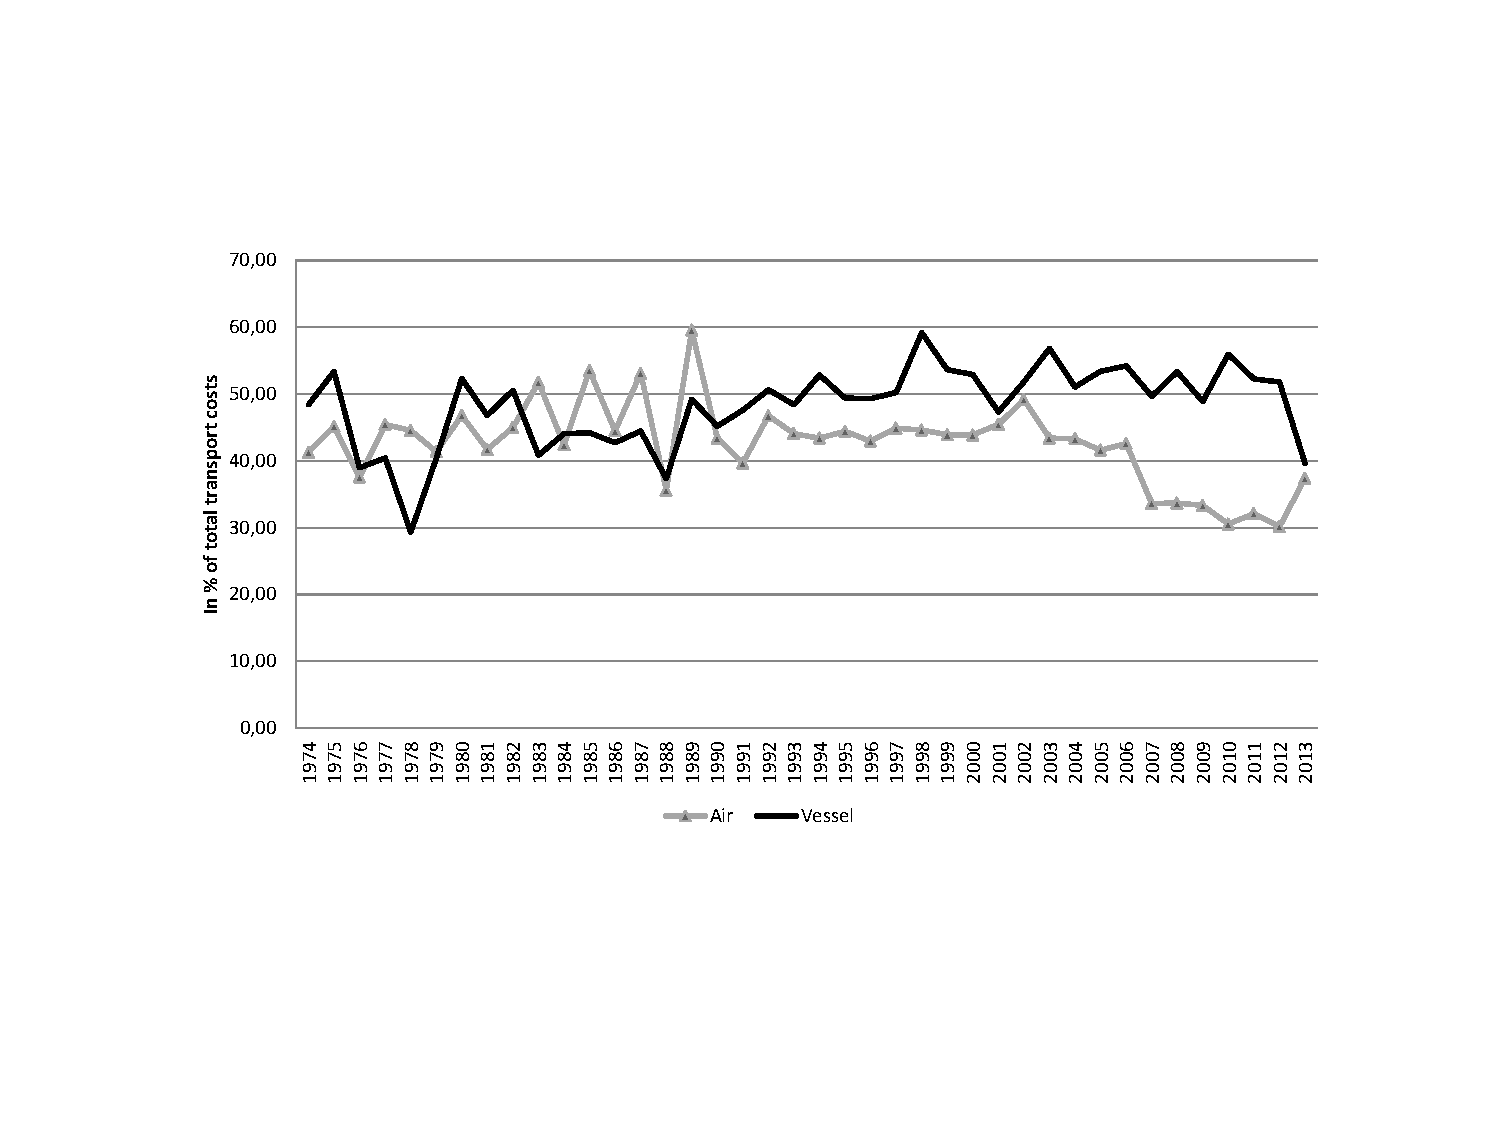
\includegraphics[width=8cm, height=5cm]{part_cout_additif.pdf}
%{\footnotesize {OECD data} }
\end{center}
\end{figure}


In both transport modes, the additive component appears of sizable importance throughout the period.
Confirming the results obtained in Table \ref{tab:summary_results}, this suggests that additive costs are neither negligible in magnitude nor an erratic phenomenon.
By contrast, they represent a sizable and structural dimension of international transport costs.
If the share of additive costs in total costs roughly amounts to 48\% (42\%) in Vessel (Air) transport on average, one can further notice that it substantially varies over time, from a minimum of 30\% to a maximum of 60\% depending on the year considered.
In the next section, we keep on investigating the importance of the (varying pattern of) additive costs, as regards with the determinants of transport costs time trends.



\section{Transport costs time trends: The role of the additive component}\label{sec:results_trends}

In this section, we investigate the trend patterns of international transport costs over time, by exploiting the time dimension of our database.
This focus is shared with part of the international trade literature, such as \cite{Lafourcade_Thisse}, \cite{hummels2007} and \cite{Behar_Venables}.
Specifically, in the same spirit as \cite{hummels2007} we investigate the underlying sources behind the downward trend of international transport costs, by identifying the respective roles of the reduction in ``pure'' transport costs and changes in trade composition effects.


\subsection{A first look at the trend patterns}

As a first step, Figure \ref{fig:Trends_in_TC} displays the evolution of total transport costs over the period, summing the additive and the ad-valorem estimated costs, expressed in percentage of the fas price,\footnote{Precisely, we use the yearly values of the estimated transport costs components averaged over the country/product dimensions (at the 3-digit level), corresponding to the numbers reported for each year in detail in the Online Appendix.
Each yearly value is obtained as: $\widehat{\tau}-1+\frac{\widehat{t}}{\widetilde{p}}$.} by transport mode for each year between 1974 and 2013.

\begin{figure}[htbp]
\caption{Trend in estimated transport costs (Yearly mean value)}
\label{fig:Trends_in_TC}
\begin{center}
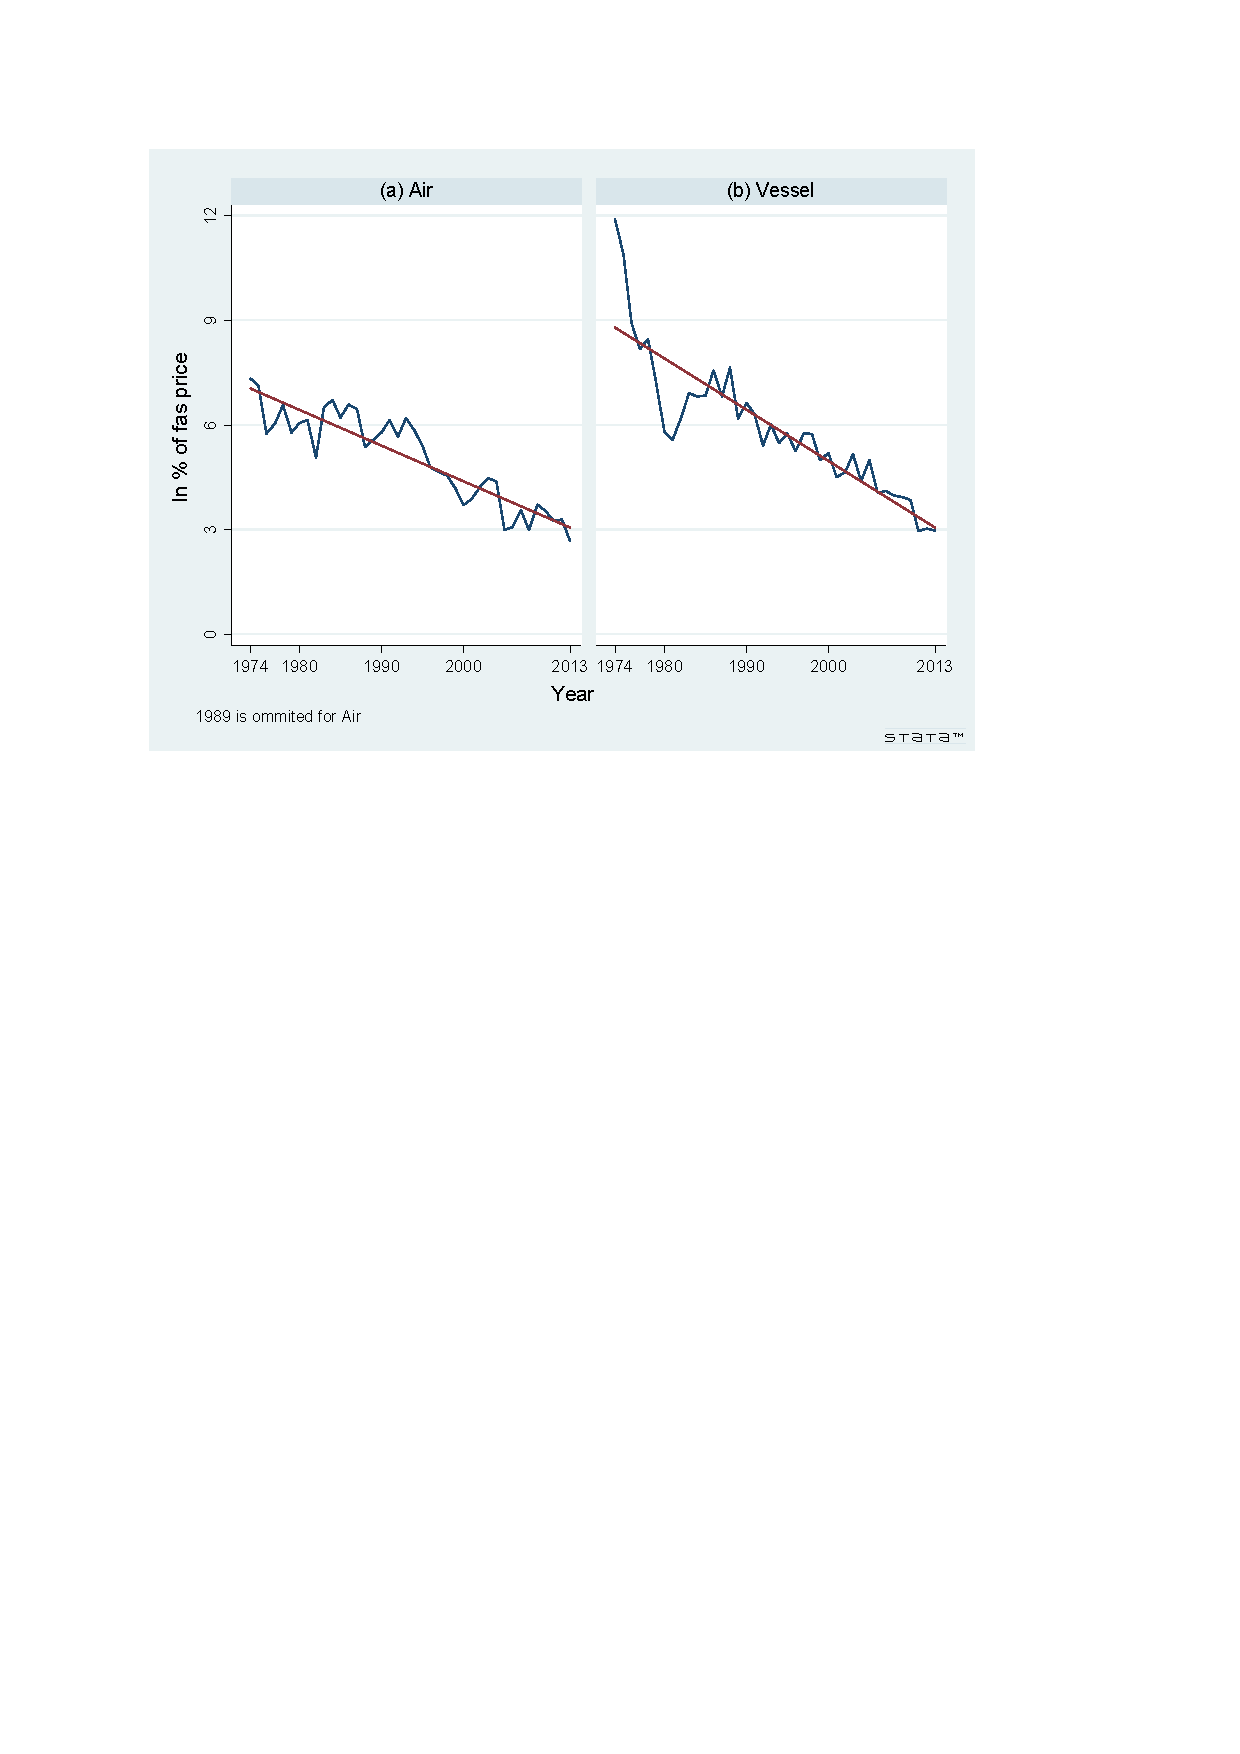
\includegraphics[width=14cm, height=6.5cm]{Figure1_Trend_of_totalTC_bymode.pdf}
\end{center}
\end{figure}


As reported in Figure \ref{fig:Trends_in_TC}, both air and vessel shipping exhibit a downward trend in overall transport costs since 1974, by -2.1\% per year for mean air transport costs and -2.0\% per year for mean ocean transport costs, implying a 50\% decrease in Air and a 60\% decrease in Vessel over the period.\footnote{One may be puzzled for by the high magnitude of estimates for the beginning of the period (until 1980 approximately) for ocean transport.
\citet{hummels2007} finds similar outcomes on tramp prices indexes, and suggests the oil shock as a likely culprit, in a context where technological progress was quicker in aviation than in vessel, allowing a better dampening of oil shocks on air freight rates.
In a related manner, one may worry that the strong decrease in transport costs documented in Figure \ref{fig:Trends_in_TC} springs from high oil-shock related transport costs in 1974.
However, computing the time trends from 1980 does not dramatically change the picture.
The yearly trend from 1980 is -2\% for mean air transport costs and -1.6\% for mean vessel transport costs.
We thus choose to exploit the whole time dimension of our database by taking 1974 as starting date of our time trend analysis.} On US data, \citet{Hummels_1999} obtains that overall transport cost declined from 6 \% to 4 \% of the import value between 1974 and 1996.
For the same years, we obtain a total decrease from 6.9 to 4.2\% in terms of the export price, on average for air shipping, and from 9.8\% to 4.8\% for ocean shipping.
Overall, our results display trends that are close to those reported by \citet{Hummels_1999}.\smallskip


Before making any definite statement about this though, it is worth emphasizing that the time trend of international transport costs depends on both the evolution of per product and per partner (``pure'') transport costs and the evolution of the composition of trade.
Total transport costs may thus have decreased over time because the share of neighboring countries in total US trade or the share of goods cheaper to transport has increased, independently of any change in transport costs \textit{per se}.
As emphasized by \citet{Hummels_1999} or \cite{hummels2007}, it is hence necessary to eliminate the composition effects of trade flows to isolate the evolution of pure international transport costs.
Specifically, Hummels's (2007) results\nocite{hummels2007} underlie the view that trade composition effects partially compensate the reduction in pure transport costs, thereby attenuating the downward trend in overall (observed) transport costs since 1974.
Our own results tend to challenge this view, as we further show.

\paragraph{A word on Hummels' methodology} At this point, let us make a brief summary of Hummels' methodology\nocite{hummels2007}.
He starts from the following specification of the ratio of destination to origin prices modelled as $p_{ikt} = \widetilde{p}_{ikt}+\frac{f_{ikt}}{ \widetilde{p}_{ikt}},$ with $f_{ikt}$ the shipping charge per-kg shipped (for a given product $k$ imported from country $i$ in year $t$).
Further, and as in \cite{hummels_skiba}, \cite{hummels2007} writes the per kg shipping charge as $f_{ikt}=\widetilde{p}_{ikt}^{1-\beta}X_{ikt}$, where $X_{ikt}$ represents other costs shifters (distance, port quality, etc.) Accordingly, his transport cost measure $TC_{ikt}$ writes down as:

\begin{equation}
TC_{ikt}\equiv \frac{p_{ikt}-\widetilde{p}_{ikt}}{\widetilde{p}_{ikt}} = \widetilde{p}_{ikt}^{-\beta}X_{ikt} \label{eq:Hummel_benchmarkeq}
\end{equation}

Notice that $\beta$ can be interpreted as the elasticity of transport costs to the export price (in absolute value).
As such, a value of $\beta = 0$ corresponds to the standard case of ``iceberg'' costs, in which transport costs are purely ad valorem.
At the other extreme, $\beta = 1$ means that all transport costs are additive.
Accordingly, the estimated value of $\beta$ can be interpreted as the share of additive costs in total transport costs.
Equation (\ref{eq:Hummel_benchmarkeq}) is the baseline specification from which \cite{hummels2007} decomposes the changes in transport costs over time between trade composition effects and changes in ``pure'' transport costs, as described with more details in Appendix \ref{app:compare_Hummels}.
In doing so, \cite{hummels2007} implicitly assumes $\beta$ constant across the triplet origin country origin/product/year.
Put differently, this means that the share of additive costs in total costs does not vary across these dimensions.

\paragraph{Challenging the $\beta$'s constancy assumption} As Figure \ref{fig:part_cout_additif} (based on the yearly estimates of transport costs averaged over the country/sector dimension) suggests, the share of additive costs is rather varying over time, in both transport modes.
%In light of this, one may wonder about the constancy of the share of additive costs along the pair product/origin country hypothesized by \cite{hummels2007}.
We investigate this point deeper by reporting the histogram of the distribution of the share of additive costs in total costs.
To do so, we start from Equation (\ref{eq:base_estimee}) with the trade costs measure on the left-hand side, from which we deduce the formulae to get the elasticity of transport costs to the export price, i.e.
$\beta$, according to:
\begin{eqnarray*}
\beta_{ikt} &\equiv& \frac{\partial TC_{ikt}}{\partial \widetilde{p}_{ikt}}\frac{\widetilde{p}_{ikt}}{TC_{ikt}} \\
&=& \frac{\widehat{t}_{ikt}/\widetilde{p}_{ikt}}{\widehat{t}_{ikt}/\widetilde{p}_{ikt}+\widehat{\tau}_{ikt}-1},
\end{eqnarray*}

\noindent making use of our first-stage estimates for both the additive and the ad-valorem components ($\widehat{t}_{ikt}$ and $\widehat{\tau}_{ikt}$).
We can henceforth rebuild the value of the elasticity on a per product-year-country basis.
The histogram of the distribution of the estimated $\beta_{ikt}$ is reported in Figure \ref{fig:histogram_beta}, in panels (a) and (b) for air and maritime transport respectively.


\begin{figure}[htbp]
\caption{Share of additive costs in total costs: Histogram}
\label{fig:histogram_beta}
\begin{center}
\begin{tabular}{cc}
%{\small (a) Air } & {\small (b) Vessel}\\
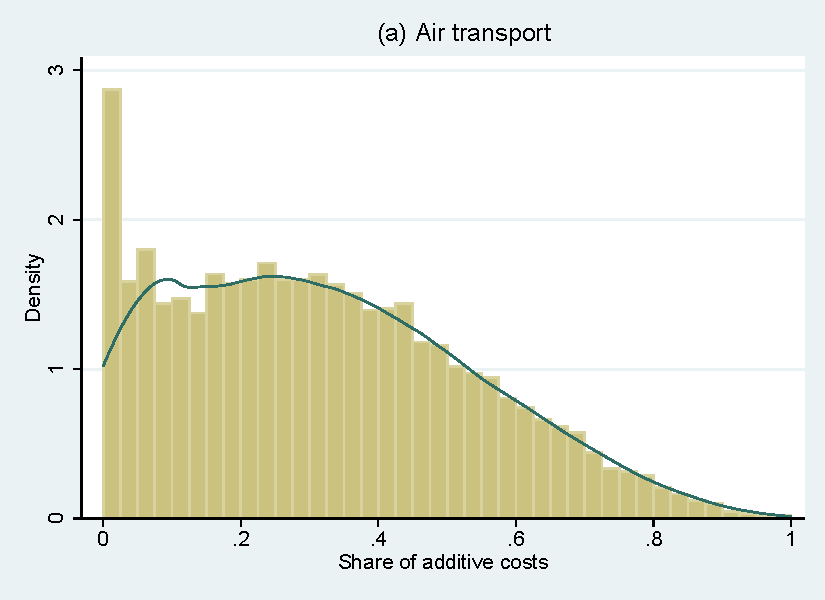
\includegraphics[width=3.0in, height=2.5in]{Etude_beta_pondere_air.pdf}
& 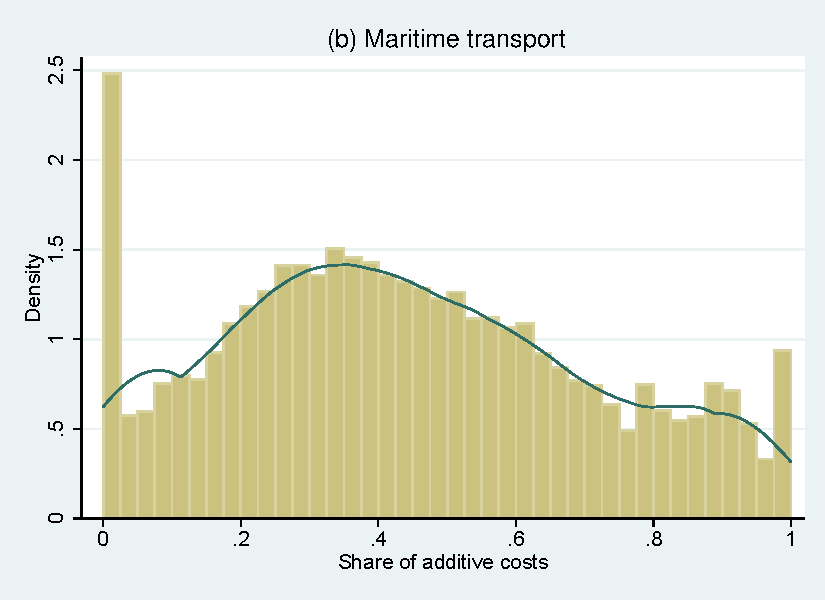
\includegraphics[width=3.0in,height=2.5in]{Etude_beta_pondere_ves.pdf} \\
\multicolumn{2}{l}{{\footnotesize Notes: Distribution of $\beta_{ikt}$ over the triplet (year,product,country), weighted by share of yearly value of flow.}}\\
\end{tabular}
\end{center}
\end{figure}

As displayed in Figure \ref{fig:histogram_beta}, for both transport modes the distribution of $\beta_{ikt}$ over the triplet (year, product, origin country) is smoothly distributed over the interval $[0,1]$, with a mode of the distribution standing around 0.3-0.4 depending of the transport mode, consistently with our previous findings.
This stands in sharp contrast with the assumption made by  \cite{hummels_skiba} or \cite{hummels2007}, which would rather imply a distribution concentrated on a single point.
Rather, this suggests that the elasticity of transport costs to the export price, or equivalently the share of additive costs in total costs, is varying across time, product and country partner.\footnote{We have checked that it is also the case when we look at the distribution over the range of origin countries or products, for a given year.
These results are not reported for sake of space saving but they are available upon request to the authors.} In the next section, we shed light on the role of this result in the analysis of the underlying sources of the overall transport costs trend patterns, between trade composition effects and pure transport costs.

\subsection{Empirical specification}

Based on the above results, we provide a decomposition of the transport costs trends between the trade composition effects and the ``pure'' transport costs time trends, that explicitly takes into account the varying share of additive costs over time, country partner and product.\footnote{See Appendix \ref{app:compare_Hummels} for a detailed comparison of Hummel's (2007) methodology and ours.} An important contribution of the paper is to show the crucial role of this (empirically relevant) assumption, as it notably modifies the conclusions relative to the role of trade composition effects.
We start with the presentation our estimation strategy before turning to the results.\smallskip

\subsubsection{Estimation strategy}

Estimation driven in Section \ref{sec:results_decomposition} provides us with the additive and ad-valorem measures of international transport costs (Equation (\ref{eq:model_IetA})), that vary over time, product and origin country (i.e., $\widehat{t}_{ikt}$ and $\widehat{\tau}_{ikt}$).
Starting from these values, for each additive and multiplicative cost component (by transport mode) we extract the pure transport cost measure by the mean of a time fixed effect.
Precisely, we extract the changes over time in the pure transport cost dimension by assuming a composition of trade flows by country partner and product that is constant throughout the period, and equal to the one observed in 1974.
We conduct the same analysis on a overall transport costs measure, built by agglomerating the two estimated components (additive and iceberg) in a unified measure of transport costs.\footnote{Note that the unfitted total transport costs are virtually the same as those reported in Figure \ref{fig:Trends_in_TC}, but reported from another perspective (basis 100 in year 1974).} The objective is to obtain six time series, all built as indices with the reference value 100 in 1974: Three time series for the unfitted transport costs measures $\{\Gamma^{add, raw}_t, \Gamma^{adv, raw}_t, \Gamma^{tc, raw}_t \}$  (additive, ad-valorem and total cost respectively), and three series for the fitted values $\{\Gamma^{add}_t, \Gamma^{adv}_t, \Gamma^{tc}_t \}$ (additive, ad-valorem and total cost respectively).

One advantage of this method is to yield measures of transport costs (fitted and unfitted) that are easily comparable between transport modes and transport cost components.
For each cost component (additive and ad-valorem) as well as for the total transport cost, comparing the unfitted measure and the fitted measure (composition effects excluded) allows to characterize if the decrease observed over the period in the unfitted series is due to trade composition effects (for instance, changes in the country partners, in the type/ quality of products traded), or if it is the pure transport costs (for instance, insurance or handling costs) that have reduced over time.
We now describe the method to extract these series (with more details provided in Appendix \ref{app:comp-effects}).


\subsubsection{Estimation method for each additive and multiplicative component}

We start describing the estimation method to extract the fitted and unfitted series for both the additive and the multiplicative components, before turning to the `total costs'' series.
\smallskip

\paragraph{Obtaining the ``pure'' transport costs component series} The empirical strategy to get the fitted transport cost measure (i.e., extracting from trade composition effect) can be described as a two-stage process.
First, we decompose the estimated measure in the three product/country/time dimensions, using fixed effects.
For the estimated ad-valorem component, we estimate the following equation:
\begin{eqnarray}
\ln(\widehat{\tau}_{ikt})&=&\delta +\underbrace{\sum_{i \neq \text{ARG}}\alpha_i.\mathbbm{1}_i}_{(a)} + \underbrace{\sum_{s(k)\neq \text{011}}\beta_{s(k)}.\mathbbm{1}_{s(k)}}_{(b)} + \underbrace{\sum_{t \neq 1974}\gamma_t.\mathbbm{1}_t}_{(c)}+\epsilon_{ikt} \label{eq:compeffects_mult}
\end{eqnarray}

\noindent where $\mathbbm{1}_i$ and $\mathbbm{1}_{s(k)}$ represent country- and sector- fixed effects.\footnote{Throughout the exercise, we consider Argentina, the sector 011 and the first year of our dataset 1974, as references for the country-, product- and year- dummies.}  Equation (\ref{eq:compeffects_mult}) is estimated using OLS, with a weighting scheme based on the value of each flow in the total value of flows the considered year.
As for the additive component, given that the sector fixed effect and the country fixed effect are additive rather than multiplicative by construction, we estimate the following equation using non-linear least squares:\footnote{For sake of notational simplicity, we do not distinguish the coefficients associated to the fixed effects between Equations (\ref{eq:compeffects_mult}) and (\ref{eq:compeffects_add}), even if they are specific to the type of transport costs considered (e.g., the series of $\gamma_t$ differs from one estimation to the other).
Note that we impose the same weighting scheme as for the OLS regression (based on the relative value of the flow).}

%, based on the additive cost series $\widehat{t}_{ikt}$ previously obtained:
\begin{eqnarray}
\ln(\widehat{t}_{ikt})&=&\ln\left( \delta + \underbrace{\sum_{i \neq \text{ARG}}  \alpha_i.\mathbbm{1}_i}_{(a)}+\underbrace{\sum_{s(k)}\beta_{s(k)}.\mathbbm{1}_{s(k)}}_{(b)}\right) + \underbrace{\sum_{t \neq 1974}\gamma_t.\mathbbm{1}_t}_{(c)}+\epsilon_{ikt} \label{eq:compeffects_add}
\end{eqnarray}
As displayed in Equations (\ref{eq:compeffects_mult}) and (\ref{eq:compeffects_add}), we decompose the estimated transport cost component in three elements: the country dimension (Term (a)), the product dimension (Term (b)) and the pure transport costs time trend (Term (c)).
Note that Equations (\ref{eq:compeffects_mult}) and (\ref{eq:compeffects_add}) preserve our specification of the ad-valorem and additive costs of Equations (\ref{eq:ad-valorem}) and (\ref{eq:add}), as we consider that the iceberg cost is the product of the country of origin and the good dimension, while the additive cost is the sum of the two dimensions.
Both equations are estimated by transport mode.\smallskip

In this exercise, we are interested in isolating the change in the time dimension of the each transport cost component.
This constitutes the second stage of our procedure.
As for the ad-valorem component defined in $[1;+\infty]$, from the estimation of Equation (\ref{eq:compeffects_mult}), we built the variable $\Gamma^{adv}_t$, for each year $t\geq 1974$, according to:
\begin{equation}
\Gamma^{adv}_t = 100.\frac {\bar{\tau}_{1974}.\exp(\gamma_t)-1} {\bar{\tau}_{1974}-1} \label{eq:comp_effects_adv}
\end{equation}

\noindent with $\bar{\tau}_{1974} = \exp(\delta +\sum_i \alpha_i +\sum_s \beta_s)$ the mean ad-valorem transport cost in 1974 (See details in Appendix \ref{app:comp-effects}).
In plain words, we measure how these costs have changed over time by blocking the composition of trade flows by product and country partners to the one observed in 1974 (the beginning of our sample).

As for the additive cost defined in $[0;+\infty]$, we built the variable $\Gamma^{add}_t$, the reference year being 1974 (ie, with $\gamma_{1974}=0$) according to:
\begin{equation}
\Gamma^{add}_t = 100.\exp(\gamma_t) \label{eq:comp_effects_add}
\end{equation}

\noindent As a result, the two series $\Gamma^{adv}_t$ and $\Gamma^{add}_t$ have a straightforward interpretation in percentage changes from the initial value of 100 for $t=1974$.


\paragraph{Obtaining the unfitted measures} The objective is to get the unfitted transport cost component (additive and multiplicative) built as an index with reference value 100 in 1974, starting from the estimated values previously obtained ($\widehat{\tau}_t$, $\widehat{t}_t$, for each year $t$ from 1974 to 2013).
To do so, we apply the simple formula to get the following indices, for the ad-valorem and the additive cost components respectively:

$$\Gamma^{adv, raw}_t = 100\times\frac{\widehat{\tau}_t}{\widehat{\tau}_{1974}},\qquad \Gamma^{add, raw}_t = 100\times\frac{\widehat{t}_t}{\widehat{t}_{1974}}$$



\subsubsection{Estimation method for the total transport cost measures}

We also build two measures of the ``total'' transport costs, that agglomerates our estimates of the two additive and ad-valorem components, for both the unfitted series and the pure transport cost series (i.e., composition effects excluded).
As for each additive and ad-valorem component, the objective is to get a measure of total transport cost changes built as an index starting from the value 100 in 1974.
Even if obeying to the same logic, we proceed slightly differently for the unfitted and the fitted measures, as we now explain.
\smallskip

\paragraph{Obtaining the unfitted total transport cost index} For each transport mode, we build the total transport cost series based on Equation (\ref{eq:base_estimee}) according to:
$$\widehat{tc}^{raw}_t= \widehat{\tau}^{adv}_t -1 + \frac{\widehat{t}_t}{\widetilde{p}_t}$$
\noindent where $\widehat{\tau}^{adv}_t$ and $\widehat{t}_t$ are the average values over the country/sector dimension estimated (conditional on a year and a transport mode), as explained in Section \ref{sec:data_method}.
Recall that $\widehat{\tau}^{adv}_t-1$ measuring the ad-valorem transport cost component and $\frac{\widehat{t}_t}{\widetilde{p}_t}$ the additive component, both expressed in percentage of the fas price.
We then transform this value in an index with basis year 1974, applying a similar formula as above (by transport mode):
$$\Gamma^{tc, raw}_t = 100\frac{\widehat{tc}^{raw}_t -1 }{\widehat{tc}^{raw}_{1974}-1}$$

\paragraph{Obtaining the fitted total transport cost index} The same logic as above applies to construct the fitted measure of total transport cost (i.e., composition effect excluded), with one notable exception though: Fitted ad-valorem and additive components have not been estimated in value, but extracted and build as indices.
In a first step then, we re-build the fitted measures of each transport cost component in value starting from these indices.
For the ad-valorem component, this can be obtained making use of Equation (\ref{eq:tcadv_compoeffect}), rewritten to get:

$$\widehat{\tau}^{pure, adv}_t = \frac{\Gamma^{adv}_t \left(\bar{\tau}_{1974}-1\right)}{100} +1$$

with $\widehat{\tau}^{pure, adv}_t \equiv \bar{\tau}_{1974}.\exp(\gamma_t)$ the yearly value of the pure (fitted) ad-valorem cost.
A similar reasoning starting from Equation (\ref{eq:tcadd_compoeffect}) gives the fitted value for the additive cost component as:

$$\widehat{t}^{pure}_t = \frac{\Gamma^{add}_t}{100}$$

with $\widehat{t}^{pure}_t \equiv \exp(\gamma_t)$ the yearly value of the pure (fitted) additive cost.


We then deduce the fitted value of the overall cost according to:
$$\widehat{tc}^{pure}_t= \widehat{\tau}^{pure, adv}_t  + \widehat{t}^{pure}_t$$

Last, we transform this (fitted) measure of total transport cost in an index with basis year 1974, applying a similar formula as above (by transport mode):
$$\Gamma^{tc}_t = 100\frac{\widehat{tc}^{pure}_t -1 }{\widehat{tc}^{pure}_{1974}-1}$$


\subsection{Characterizing the time trends in transport costs}
Figure \ref{fig:totalTC_compeffects_excl} reports the results for all types of goods.\footnote{In the Online Appendix, we report the results at a more disaggregated level, distinguishing between primary and manufacturing goods.} In panels (a), (b) and (c) we report the time changes of the ad-valorem costs, the additive costs and the total costs respectively, for Air transport (starting from the reference value 100 in 1974).
Panels (d), (e) and (f) report the results for Vessel.
In each panel, we report the evolution of transport costs for both the unfitted (plain blue line) and the fitted (dotted red line) measures.


\begin{figure}[htbp]
\caption{Transport costs (with and without composition effects)}
\label{fig:totalTC_compeffects_excl}
\begin{center}
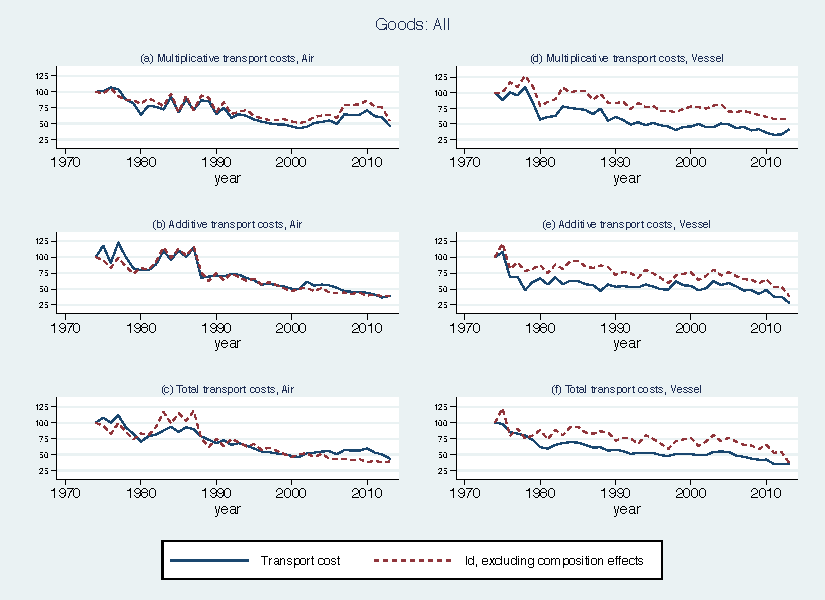
\includegraphics[height=4in]
{graph_composition_all.pdf}
\end{center}
\end{figure}

Three main results emerge from Figure \ref{fig:totalTC_compeffects_excl}.
First, in accordance with Figure \ref{fig:Trends_in_TC}, we find that international transport costs have substantially decreased over the period, for both transport modes (Panels (c) and (f)).
International transport costs were reduced by 50\% between 1974 and 2013 in air shipping, and by 60\% in maritime shipping.
This stands in line with the related literature (see \citealp{Hummels_1999}, \citealp{Lafourcade_Thisse}).
Second, the magnitude of the decrease is roughly of the same order for both for the ad-valorem and the additive components (Panels (a), (b), (d) and (e)).
Further, the transport cost reduction is much smoother in maritime transport, while air transport shows more volatility in the trend pattern, in particular in the 1980s and the 2000s.
Third, and most importantly, we find that composition effects do not play a major role in accounting for the time trend of overall transport costs.
Inspecting the panels of Figure \ref{fig:totalTC_compeffects_excl} for Air transport (panels (a) to (c)), we do not find much evidence of a substantial trend difference between the unfitted transport costs measure and the pure transport costs.
For all three series (additive, ad-valorem and overall transport costs), the dotted and the plain line follow closely, almost every year throughout the period.
Air transport costs were reduced by 50\% between 1974 and 2013, and this is mainly attributable to a reduction in the transport costs ``per se''.
Composition effects are stronger in vessel transport, for all three series (Figure \ref{fig:totalTC_compeffects_excl}, panels (d) to (f)): they amplify the reduction in ``pure'' transport costs at the beginning the period, in the 1970s (the dotted line is below the plain line, and the gap is increasing). Afterwards, the dotted line remains below the plain line, but the gap between the two remains roughly constant across years, indicating that the amplification effect does not strengthen anymore: both trends are very similar.
Considering the raw series (plain line), maritime transport costs have decreased by 60\% over the period, which can be decomposed in a 50\% decrease in transport costs ``per se'' (dotted line), and a 10\% reduction that comes from composition effects (the difference of the two).
This is particularly the case for the multiplicative component (panel (d)).\smallskip




\subsection{Time trends in transport costs and the modeling of the additive component}

The last results stand in sharp contrast with \citet{hummels2007}, who obtains that trade composition effects do matter, as they partially offset the reduction in the pure transport costs for both air and maritime shipping.
If anything, we find the opposite result here: Trade composition effects do not matter much in accounting for the downward trend of observed international transport costs, and when they do, they tend to amplify (rather than reduce) the downward pattern.
This drives us to investigate this difference further.
As we explain in more details in Appendix \ref{app:comp-effects}, our empirical strategy differs from \cite{hummels2007} in one main dimension.
Our characterization of the time trends in transport costs starts from our estimates of both the additive and the ad-valorem components (obtained in Section \ref{sec:results_decomposition}), as well as for the overall transport cost (rather than the actual cif-fas price gap).
Consequently, our methodology lets the ratio between the additive and the ad-valorem components of transport costs vary over the three time-product-partner country dimensions.
%By contrast, \cite{hummels2007} does not take into account the changes in the additive transport cost component, attributing this to a change in the composition of the bundle over time (per country-commodity).
This turns out to be of primary importance in the disentangling in the time trend of transport costs, between what comes from the trade composition effects and what comes from changes in the pure transport cost dimension, as we show below.

To establish this point clearly, we replicate the method adopted by \cite{hummels2007} exposed above on our database (which is the same as his until 2004).
The results are reported in Figure \ref{fig:comp_effects_as_in_Hummels}.
The dotted line labeled ``expenditure/import value'' represents the unfitted measure of transport costs ($TC_t$ in the above terminology) and the plain line labeled ``fitted ad-valorem rate'' is the measure of ``pure'' transport costs, i.e.
composition effects excluded ($\widehat{TC}_t$).
In Panels (a) (for Air) and (b) (for Vessel), we report the transport costs measures (fitted and unfitted) expressed as a percentage of the export price, as in \cite{hummels2007}.\footnote{Unsurprisingly, this stands in accordance with \citeh{hummels2007} results, see his Figures 5 (for Air) and 6 (for Vessel).} To ease the interpretation of the trends, we express them as indices with the reference value 100 in 1974, in Panels (c) and (d) for Air and Vessel respectively.

\begin{figure}[htbp]
\caption{Characterizing the time trends: Applying Hummel's (2007) method }
\label{fig:comp_effects_as_in_Hummels}
\begin{center}
\begin{tabular}{cc}
{\small (a) Ad-valorem Air Freight} & {\small (b) Ad-valorem Vessel Freight}\\
\multicolumn{2}{c}{{\small In percent of the export price}} \\
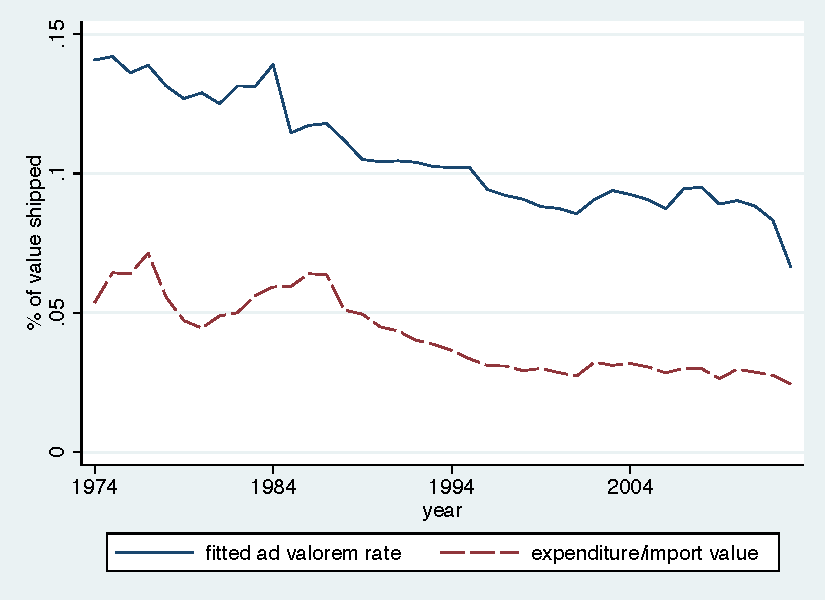
\includegraphics[width=2.5in, height=1.8in]{figure5_comme_hummels.pdf}
& 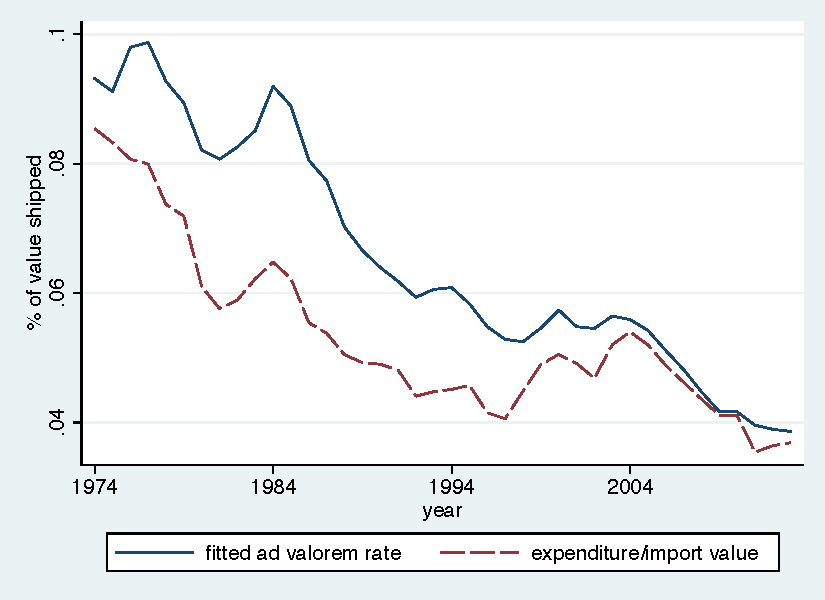
\includegraphics[width=2.5in,height=1.8in]{figure6_comme_hummels.pdf} \\
{\small (c) Ad-valorem Air Freight} & {\small (d) Ad-valorem Vessel Freight}\\
\multicolumn{2}{c}{{\small As indices with reference value 100 in 1974} }\\
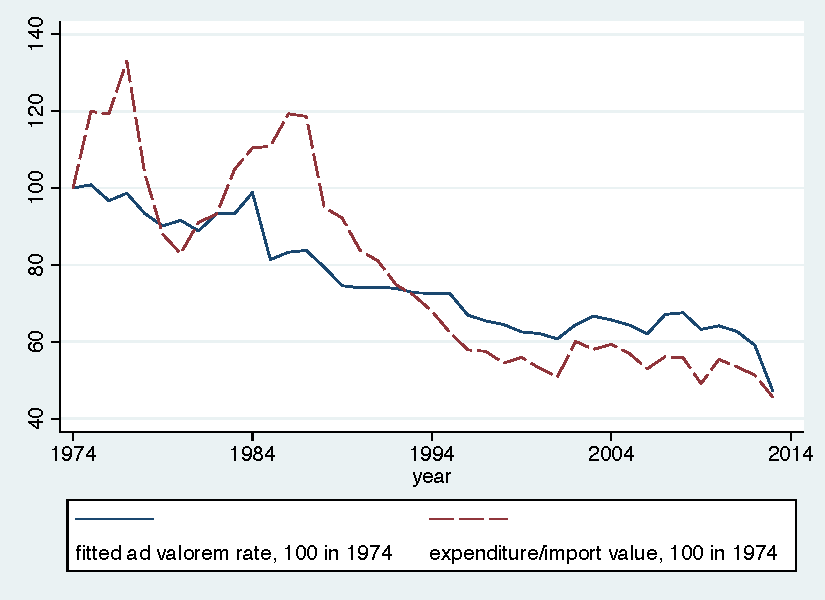
\includegraphics[width=2.5in, height=2in]{figure5_comme_hummels_base100.pdf}
& 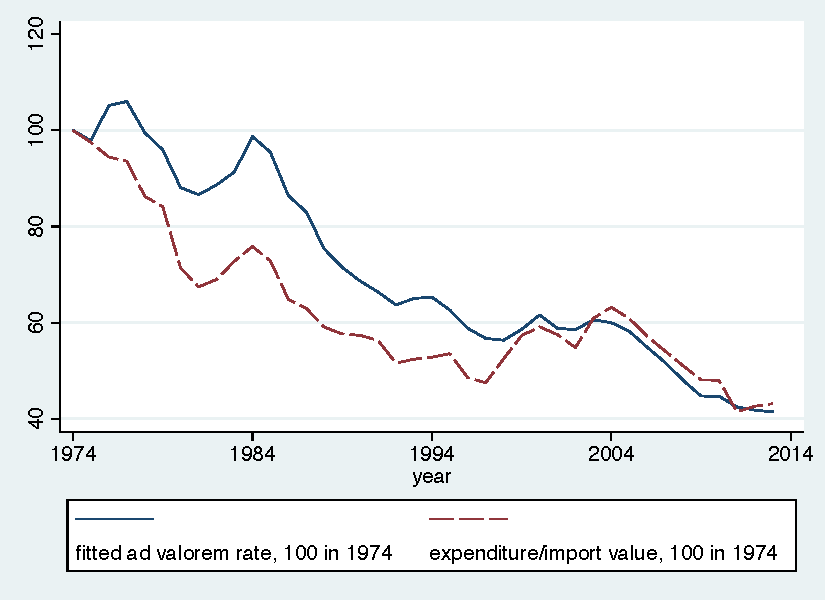
\includegraphics[width=2.5in,height=2in]{figure6_comme_hummels_base100.pdf} \\
\end{tabular}
\end{center}
\end{figure}

These results stand in sharp contrast with the ones obtained with our methodology and reported in Figure \ref{fig:totalTC_compeffects_excl}.
Applying \citeh{hummels2007} method, we find that the composition effects tend to partly offset the decrease in transport costs in both air and vessel shipping, as the downward trend is of higher magnitude for the fitted rate (plain line) than the unfitted rate (dotted line), especially for Vessel (Panel (d)).
Yet, this result is overturned when we allow for more flexibility in the role of the additive component, as pointed in Figure \ref{fig:totalTC_compeffects_excl}, panels (c) and (f).\medskip


Assuming a varying share of the additive component over time, product and country partner indeed modifies the decomposition of the trend reduction of transport costs between the one attributable to trade composition effects and the reduction in the ``pure'' transport costs.
In both air and vessel transports, we thus find that this last dimension is the main driver of the reduction of international transport costs observed over time, in particular in air transport.
Complementing the findings of Section \ref{sec:results_decomposition}, these results point out the importance of integrating the additive dimension of international transport costs, here in view of characterizing their time trends.

\section{Robustness analysis \label{sec:robustness}}

\subsection{Robustness to the separability assumption}
In this section, we provide a robustness analysis to the separability assumption of country-good fixed effects, that considers (following so \citealp{Irrazabal_2015}) that both the ad-valorem and the additive costs are separable between the origin country ($i$) and the product ($s(k)$) dimensions.
That is, we relax Equations (\ref{eq:ad-valorem}) and (\ref{eq:add}) to rather model $t_{is(k)}$ and $t_{is(k)}$ (on a yearly/transport mode basis).
Yet, this comes at the cost of having to estimate a much larger number of fixed effects (for approximatively 200 countries of origin and 200 sectors at the 3-digit level, this means estimating 40,000 versus 400 fixed effects, per year and per transport mode), making the estimation (all the more given our non-linear setting) intractable in practice.
This drives us to conduct the analysis on a sub-sample of trade flows, upon which two estimations are conducted (for every year and each transport mode): with the separability assumption (Equations (\ref{eq:ad-valorem}) and (\ref{eq:add}) hold, our baseline case) and without.
For each year and transport mode, we select the countries ($i$) and the products (at the 3-digit level, $s(k)$) that constitute 80\% of the total value of trade flows. Table \ref{tab:robustness_separability} reports a summary of the results, considering the average estimated values over the period (by transport mode).

\begin{table}[htbp]
  \centering
  \caption{Robustness to the separability assumption (Average over the period) - restricted sample}
\begin{center}
    \begin{tabular}{lcc|cc}
    \hline \hline
    \multicolumn{5}{c}{Mean value over 1974-2013} \\
 \multicolumn{5}{c}{3 digits} \\    \hline \hline
   Mode  & \multicolumn{2}{c|}{Air} & \multicolumn{2}{c}{Vessel} \\ \hline
   Separability & No  & Yes (baseline) & No & Yes (baseline)\\ \hline
    \multicolumn{5}{l}{\textit{Additive term} ($\widehat{t}/\widetilde{p}$.
in \%)}  \\
    Mean  & 1.76 & 1.96 & 2.61 & 2.99 \\
    Median &0.65 & 0.84 &1.83 & 2.23 \\ \hline
    \multicolumn{5}{l}{\textit{Ad-valorem term} ($\widehat{\tau}$, in \%)}\\
    Mean  & 1.04 & 0.94 & 2.43 & 2.40 \\
    Median & 0.56 & 0.83 & 2.06 & 2.04 \\ \hline
\multicolumn{5}{l}{\textit{Share of additive costs in total costs (in \%)}} \\
    Mean  & 62.8  & 67.5  & 51.8  & 55.4 \\
    Median & 54.1  & 50.5  & 47.0  & 52.2 \\  \hline
 \textit{Diagnostic test} & & &  &  \\
    %$R^2$    & \multicolumn{1}{c}{0.80} & \multicolumn{1}{c}{0.68} & \multicolumn{1}{c}{0.67} & \multicolumn{1}{c}{0.45} \\
    %SER   & \multicolumn{1}{c}{0.57} & \multicolumn{1}{c}{0.72} & \multicolumn{1}{c}{0.53} & \multicolumn{1}{c}{0.69} \\
    AIC criteria & 4657.60 & 4654.23 & 10744.83 & 10690.80 \\ \hline
    %Log-likelihood & \multicolumn{1}{c}{-1757.75} & \multicolumn{1}{c}{-2258.24} & \multicolumn{1}{c}{-4018.51} & \multicolumn{1}{c}{-5220.00} \\ \hline
\# observations & 2381 & 2381 & 2798 & 2798 \\
\# origin country & 13.4 & 13.4 & 19.8 & 19.8 \\
\# products & 25.5 & 25.5 & 53 & 53 \\ \hline \hline
    \end{tabular}%
\end{center}
\parbox[l]{10cm}{\tiny{Notes: Estimations are performed on a restricted sample, based on the following rule: for each year and transport mode, we select the countries ($i$) and the products (at the 3-digit level, $s(k)$) that constitute 80\% of the total value of trade flows.
The additive term is expressed in fraction of fas price.
($^{\ast \ast}$): 1989 omitted in 3-digit estimation for air.}}
\label{tab:robustness_separability}
\end{table}


Three main comments can be made.
First, the subset of big trade flows we are considering (around 8\% of our initial sample, but 80\% of the total value of aggregated trade) involve a higher share of additive costs: between 52 and 67\% of total costs on average, versus 40 to 50\% on the whole sample.
%JH: la phrase suivante est en contradiction avec celle qui suit encore juste après: "Second, assuming that country/product fixed effects are separable in these two dimensions tends to overestimate the value and the share of the additive costs."
Second, both models provide a similar quality of fit of the regression (once we take into account the number of right-hand side variables) as the AIC criteria displays very close values in both models (conditional on transport mode).
Third, the estimated values remain of similar magnitude under both separability and non-separability assumptions, even if one can note that under the separability assumption, the share of additive costs seems slightly biased upward, at least for averages over the period - the picture is reversed for medians.
Before jumping to the conclusion that our results are robust to the separability assumption though, we investigate this comparison deeper on a year-to-year basis, as reported in Figure \ref{fig:robustesse_non_separe}.
Precisely, Figure \ref{fig:robustesse_non_separe} displays the results for Air transport in panel (a) and for maritime transport in panel (b).
In each case, the estimated values (as well as the fitted regression line) under both separability (baseline) and non-separability, for the additive term (upper panel) and the ad-valorem term (lower panel).


\begin{figure}[htbp]
\caption{Robustness to the separability assumption (Year-to-year basis)}
\label{fig:robustesse_non_separe}
\begin{center}
\begin{tabular}{cc}
{\small (a) Air Freight} & {\small (b) Vessel Freight}\\
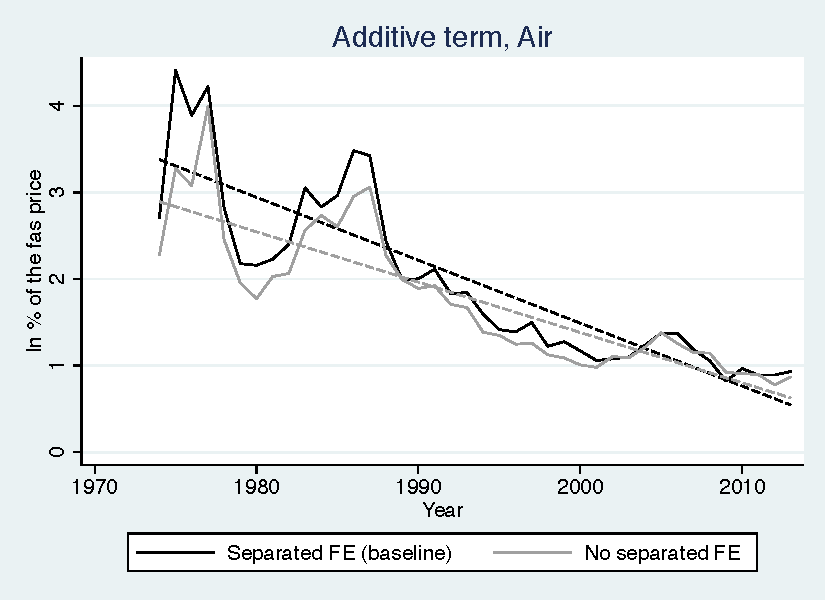
\includegraphics[width=2.5in, height=2in]{graph_robustesse_ns_mp_terme_A_air.pdf}
& 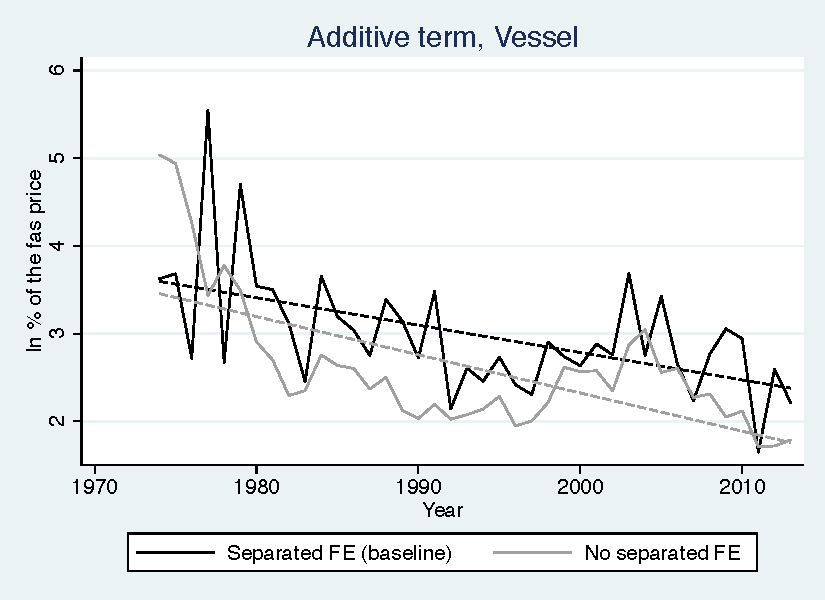
\includegraphics[width=2.5in,height=2in]{graph_robustesse_ns_mp_terme_A_ves.pdf} \\
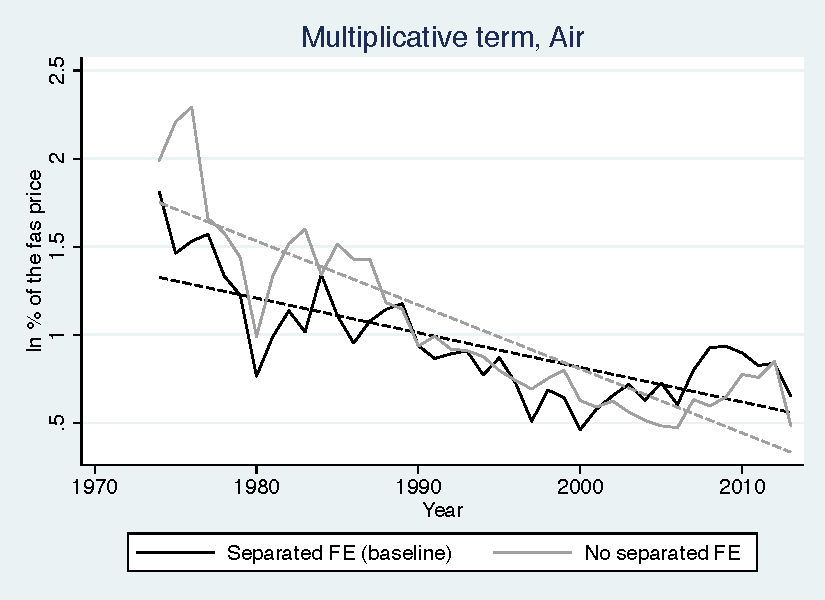
\includegraphics[width=2.5in, height=2in]{graph_robustesse_ns_mp_terme_I_air.pdf}
& 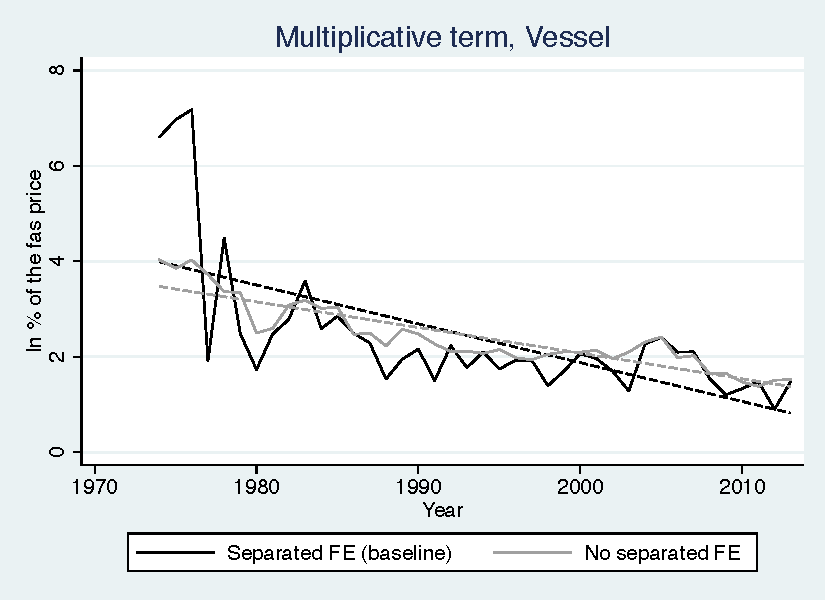
\includegraphics[width=2.5in,height=2in]{graph_robustesse_ns_mp_terme_I_ves.pdf} \\

\end{tabular}
\end{center}
\end{figure}

In line with Table \ref{tab:robustness_separability}, the results reported in Figure \ref{fig:robustesse_non_separe} confirm that the separability assumption (retained in our baseline estimation) tends to overestimate the value of the additive cost component (and underestimate the value of the ad-valorem cost).
However, they also show that the difference is quantitatively small; further, and most importantly, whatever the transport mode and for both types of transport costs, the trend patterns of international transport costs are very similar to the one another, whether they are estimated under the separability assumption or not.
Along with the quality of fit diagnosis, this confirms the robustness of our estimation results to this assumption.

As an ultimate check, we investigate whether the varying pattern over time/country of origin/product pointed out in Section \ref{sec:results_decomposition} is also robust to the separability assumption.
To this aim, we replicate Figure \ref{fig:histogram_beta} on the reduced sample for both specifications of separable (baseline) and non-separable fixed costs.
Figure \ref{fig:histogram_beta_robustness} reports the histogram of the distribution of the elasticity of transport costs to the export price ($\beta_{ikt}$, for Air transport (top panel) and for maritime transport (bottom panel) under the baseline specification (Panels (a, (c))) and the non-separability scenario (Panels (b), (c)).


\begin{figure}[htbp]
\caption{Histogram of the share of additive costs in total costs (restricted sample)}
\label{fig:histogram_beta_robustness}
\begin{center}
\begin{tabular}{cc}
\multicolumn{2}{c}{Air transport} \\
{\small (a) Separability (baseline)} & {\small (b) Non-separability}\\
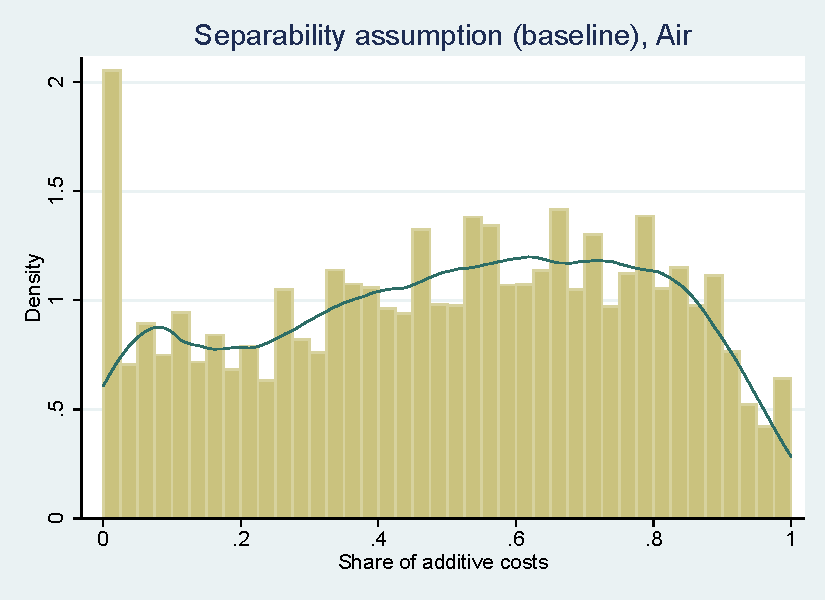
\includegraphics[width=7cm, height=5cm]{Etude_beta_pond_sitc2separe_air.pdf}
& 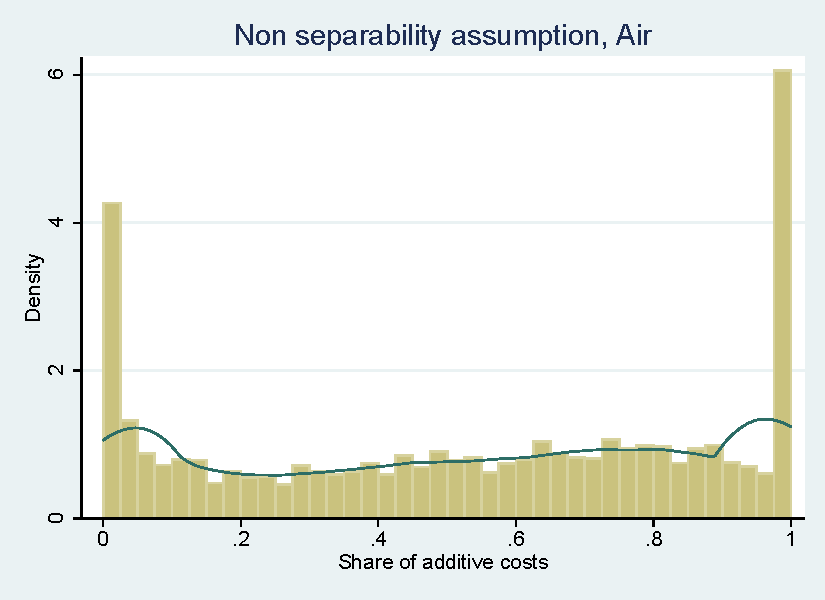
\includegraphics[width=7cm, height=5cm]{Etude_beta_pond_sitc2ns_air.pdf} \\
\multicolumn{2}{c}{Maritime transport} \\
{\small (c) Separability (baseline)} & {\small (d) Non-separability}\\
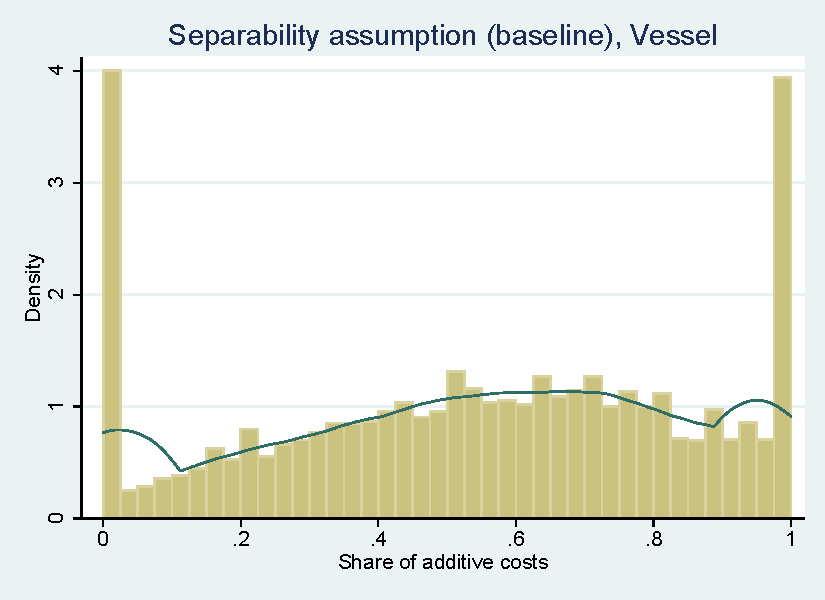
\includegraphics[width=7cm, height=5cm]{Etude_beta_pond_sitc2separe_ves.pdf}
& 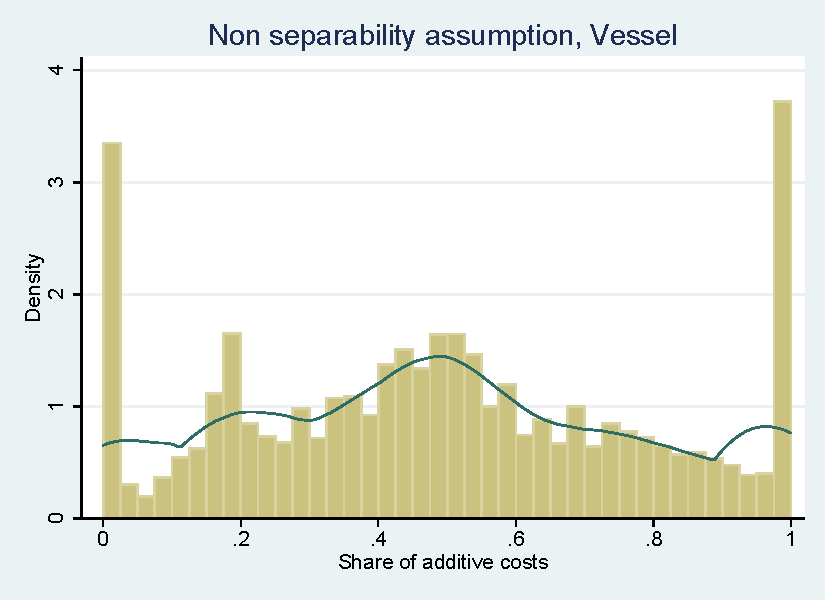
\includegraphics[width=7cm, height=5cm]{Etude_beta_pond_sitc2ns_ves.pdf} \\
\multicolumn{2}{l}{{\footnotesize Notes: Distribution of $\beta_{ikt}$ over the triplet (year-product-country), weighted by share of yearly value of flow.}}\\
\end{tabular}
\end{center}
\end{figure}

Similarly as for the whole sample (Figure \ref{fig:histogram_beta}), for both transport modes the distribution of $\beta_{ikt}$ over the triplet (year, country of origin, product) appears smoothly distributed over the interval $[0,1]$, whatever the assumption regarding the specification of fixed effects.
Relaxing the assumption that fixed effects are separable between the two country and product dimensions does not alter qualitatively our conclusion, that the elasticity of transport costs to the export price (or the share of additive costs in total transport costs), is strongly varying over time, countries of origin and products.
As a consequence, this also provides an indirect robustness check to the results regarding the trend decomposition provided in Section \ref{sec:results_trends}, that establish that the decline of ``pure'' transport costs lies as main reason for the decrease of overall transport costs observed over time.


\subsection{Robustness to the weighting scheme }

As discussed in Appendix \ref{app:comp-effects}, one source of difference between our methodology and \citet{hummels2007}'s dwells on the weighting scheme used to obtain the evolution of the pure transport costs over time.
In this section, we provide a robustness test to this difference of treatment.\smallskip

When aggregating the trade cost measure over the product/country ($i,k$) dimension, \cite{hummels2007} takes the unweighed average value over the $i,k$ dimension, which implicitly attributes a weight equal to 1 to each flow.
Our benchmark specification  (at the root of Figure \ref{fig:totalTC_compeffects_excl}) proceeds differently, as each flow is weighted by its relative value in total trade flows observed in 1974.
In this section, we check that this difference of treatment is not responsible for the difference of results relative to the role of the trade composition effects, that we rather attribute to the modeling of the additive component.

To this aim, we rebuild the fitted values for each of of our transport cost measures (ad-valorem, additive and overall) applying \citet{hummels2007}'s weighting scheme (i.e., taking the unweighed average value over the $i,k$ dimension), which we then express as indices, with the reference value 100 in 1974.
The results are reported in Figure \ref{fig:compeffects_robustness}.

\begin{figure}[htbp]
\caption{Transport cost time trends: Robustness to the weighting scheme}
\label{fig:compeffects_robustness}
\begin{center}
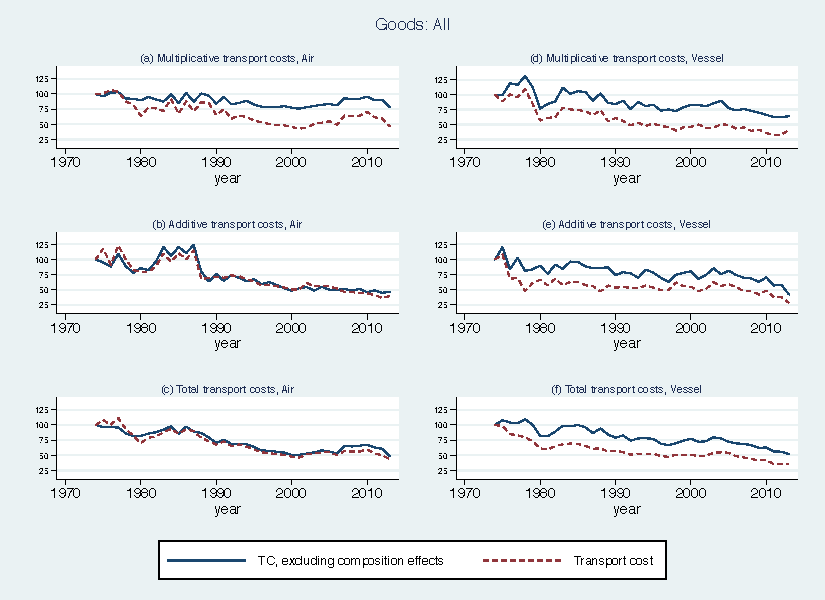
\includegraphics[height=8cm]
{graph_composition_all_np.pdf}
\end{center}
\end{figure}

The comparison of Figure \ref{fig:compeffects_robustness} (applying \citealp{hummels2007}'s weighting scheme) and Figure \ref{fig:totalTC_compeffects_excl} (applying our weighting scheme) drives two comments.
First, differences do show up, in particular for the multiplicative component of Air transport.
This suggests that the weighting scheme is not innocuous in the time trend decomposition exercise.
However, Figure \ref{fig:compeffects_robustness} also shows that the composition effects have contributed to strengthen the decrease in the ``ceteris paribus'' transport costs in Air transport (in Figure \ref{fig:compeffects_robustness}, panel (a), overall transport costs have decreased more that the fitted component), in accordance with the conclusions drawn from Figure \ref{fig:totalTC_compeffects_excl}, rather than partly offsetting this decline, as argued by \cite{hummels2007}.
This confirms that it is the functional form and precisely the modeling of the additive component, rather than the weighting scheme, that is key in understanding the underlying determinants of the overall transport costs time trends, as pointed out in Section \ref{sec:results_trends}.



\section{Conclusion \label{sec:conclu}}

This paper empirically studies the magnitude of additive costs in international transport costs, by exploiting the differences between the import and the export prices.
Using SITC 3 and 4- digit cif-fas unit values taken from the US import database over 1974-2013, we estimate the two components (additive and ad-valorem) of transport costs, by transport mode (air or ocean).
Two main findings emerge from our results.
First, we provide a quantitative measure of both the additive and the ad-valorem transport cost.
We find that additive costs are quantitatively sizable: They amount to 2.8\% of the export price unit values for ocean shipping, 1.8\% for air transport.
This is slightly lower that the estimated values for the d-valorem costs, around  2.5\% (vessel) and 3.2\% (air) as mean values over 1974-2013.
Further, modeling the additive component significantly improves the quality of fit of the regression.
Second, we show the importance of integrating the additive component in accounting for the time trend of international transport costs.
Allowing for a varying share of additive costs in product/country/time dimension, we find that the decrease of international transport costs observed in the data is mostly attributable to a reduction in the \textit{pure} transport costs, with trade pattern composition effects playing a small role.
If anything, trade composition effects have contributed to amplify the reduction in the pure transport costs in maritime transport.
In both aspects, our results point the importance of the additive component in accounting for international transport costs.

Our results could be extended in two main ways.
On the empirical side, one may want to go deeper in the structural determinants of (pure) transport costs, i.e.
identify the respective roles of handling costs, insurance and freight at the root of the gap between export and import prices.
On the theoretical side, our results can be used to explore the role of additive costs in shaping international trade flows in an international trade theory perspective and in affecting the international transmission of business cycles.
This is left for further research.



\newpage
\bibliographystyle{essaien}
\bibliography{biblio}


\newpage


\appendix

\clearpage

%\appendix
\setcounter{table}{0}
\renewcommand{\thefigure}{A.\arabic{figure}}
\renewcommand{\thetable}{A.\arabic{table}}


\section{Data Appendix \label{app:data}}


The Customs value is the value of imports as appraised by the U.S.
Customs and Border Protection in accordance with the legal requirements of the Tariff Act of 1930, as amended.
This value is generally defined as the price actually paid or payable for merchandise when sold for exportation to the United States, excluding U.S.
import duties, freight, insurance, and other charges incurred in bringing the merchandise to the United States.
The term ``price actually paid or payable'' means the total payment (whether direct or indirect, and exclusive of any costs, charges, or expenses incurred for transportation, insurance, and related services incident to the international shipment of the merchandise from the country of exportation to the place of importation in the United States) made, or to be made, for imported merchandise by the buyer to, or for the benefit, of the seller.
In this respect, the ``custom value'' corresponds to the fas price (``free-alongside'' price) delivered by the seller.
More information on this database is available at: \url{http://www.census.gov/foreign-trade/reference/products/catalog/fl_imp.txt}.

The import charges represent the aggregate cost of all freight, insurance, and other charges (excluding U.S.
import duties) incurred in bringing the merchandise from alongside the carrier at the port of exportation in the country of exportation and placing it alongside the carrier at the first port of entry in the United States.
In the case of overland shipments originating in Canada or Mexico, such costs include freight, insurance, and all other charges, costs and expenses incurred in bringing the merchandise from the point of origin (where the merchandise begins its journey to the United States in Canada or Mexico to the first port of entry.

The cif (cost, insurance, and freight) value represents the landed value of the merchandise at the first port of arrival in the United States.
It is computed by adding ``Import Charges'' to the ``Customs Value'' (see definitions above) and therefore excludes U.S.
import duties.

\clearpage
\setcounter{table}{0}
\setcounter{figure}{0}
\renewcommand{\thefigure}{B.\arabic{figure}}
\renewcommand{\thetable}{B.\arabic{table}}

\section{Estimation at the 3-digit classification level \label{app:more_results}}

\subsection{Transport costs estimates: More detailed results}

In this section, we report more detailed results for the estimates for international transport costs, by transport mode on a yearly basis, when either additive costs are included in the estimation (Equation (\ref{eq:model_IetA})) or not (Equation (\ref{eq:model_nlI})), under our benchmark sectoral classification level (3 digit).
Precisely, we complement the results displayed in Table \ref{tab:summary_results} by reporting the estimates of international transport costs for a sample of years over 1974-2013, when the degree of classification retained ($s$) is at the 3-digit classification level.
Table \ref{tab:result_air_3d_detail} reports the results for Air transport.
The results for Vessel transport are displayed in Table \ref{tab:result_ves_3d_detail}.

%\todo{Changer\begin{table}[htbp]
\begin{table}[htbp]
  \caption{Air: Transport costs estimates, 3-digits (selected years)}
\begin{center}
    \begin{tabular}{l|ccccccc}
\hline\hline
Year & 1974  & 1980  & 1990  & 2000  & 2004 & 2010  & 2013   \\
\hline
\multicolumn{8}{l}{\textbf{Model (a) - With only Ad-Valorem TC} ($\widehat{\tau}^{ice}-1$, in \%)}     \\
\hline
Mean  & 6.9& 5.4 &5.0 & 3.6 & 4.0 & 4.2 & 3.4  \\
Median & 5.4 & 3.8 & 4.4 & 2.5 & 2.9 & 3.4 & 2.9  \\
%Standard Error & 0.052 & 0.049 & 0.039 & 0.033 & 0.037 & 0.024 \\
\hline
\multicolumn{8}{l}{\textbf{Model (b) - With Additive \& Ad-Valorem TC}}    \\
\hline
\multicolumn{8}{l}{\textit{Ad-valorem term} ($\widehat{\tau}^{adv}-1$, in \%)}  \\ \hline
Mean & 3.6 & 2.3 & 2.4 &1.7 & 1.9 & 2.6 & 1.7  \\
Median & 2.7 & 1.6 & 1.6 & 1.2 & 1.4 & 2.2 & 1.7 \\
%Standard Error & 0.032 & 0.025 & 0.021 & 0.016 & 0.023 & 0.012  \\

\hline
\multicolumn{8}{l}{\textit{Additive term} ($\widehat{t}/\widetilde{p}$, in \%)}     \\ \hline
Mean & 2.6 & 2.0 & 1.8 & 1.3 & 1.5 & 1.1 & 1.0  \\
Median & 1.1 & 0.5 & 0.8 & 0.5 & 0.6 & 0.4 & 0.5  \\
%\multicolumn{1}{l}{Standard Error} & 0.040 & 0.041 & 0.033 & 0.028 & 0.024 & 0.020  \\
\hline
\# observations & 14,955 & 16,118 & 24,958 & 35,027 & 36,990 & 40,279 & 39,351  \\
\hline\hline
\multicolumn{8}{l}{\parbox[l]{11cm}{ \vspace{7pt}\scriptsize{Notes: TC = Transport Costs.
Statistics are obtained weighting each observation by its share in trade (mode-dependent).
Additive term expressed in fraction of fas price.}}}
\end{tabular}%
\end{center}
\label{tab:result_air_3d_detail}
\end{table}%

\begin{table}[htbp]
  \centering
  \caption{Vessel: Transport costs estimates, 3 digit (selected years)}
\begin{center}
    \begin{tabular}{l|ccccccc}
   \hline\hline
Year         & 1974  & 1980  & 1990  & 2000  & 2004 & 2010  & 2013   \\
 \hline
   \multicolumn{8}{l}{\textbf{Model (a) - With only Ad-Valorem TC} ($\widehat{\tau}^{ice}-1$, in \%)}  \\
   \hline
Mean  & 9.8 & 6.5 & 5.7 & 5.1 & 5.4 & 4.0 & 3.6  \\
Median & 9.6 & 5.5 & 4.6 & 4.9 & 5.1  & 3.6 & 3.3  \\
%Standard Error & 5.3 & 4.0 & 3.2 & 2.8 & 2.0 & 1.8  \\
\hline
\multicolumn{8}{l}{\textbf{Model (b) - With Additive \& Ad-Valorem TC}}    \\
\hline
\multicolumn{8}{l}{\textit{Ad-valorem term ($\widehat{\tau}^{adv}-1$, in \%)} } \\
\hline
Mean  & 5.4 & 3.1 & 3.3 & 2.5 & 2.7 & 1.9 & 2.2 \\
Median & 4.9 & 2.4 & 2.8 & 2.1 & 2.8 & 1.8 & 1.8  \\
%Standard Error & 0.041 & 0.023 & 0.022 & 0.021 & 0.018 & 0.018  \\
\hline
\multicolumn{8}{l}{\textit{Additive term ($\widehat{t}^{add}/\widetilde{p}$, in \%)}}  \\
\hline
Mean  & 5.1 & 3.4 & 2.7 & 2.8 & 2.9 & 2.5 & 1.5  \\
Median & 2.9 & 2.3 & 1.7 & 2.2 & 1.9 & 1.9 & 0.8 \\
%Standard Error & 0.085 & 0.046 & 0.040 & 0.043 & 0.025 & 0.020 \\
\hline
 \# observations & 19,007 & 17,356 & 28,383 & 36,090 & 37,757 & 37,748 & 38,473 \\
\hline\hline
\multicolumn{8}{l}{\parbox[l]{11cm}{ \vspace{7pt}\scriptsize{Notes: TC = Transport Costs.
Statistics are obtained weighting each observation by its share in trade (mode-dependent).
Additive term expressed in fraction of fas price.}}}
\end{tabular}%
\end{center} \label{tab:result_ves_3d_detail}
\end{table}%


\subsection{Assessing the importance of additive transport costs \label{app:diagnostic_test}}

In this section, we explore the performances of each type of model (with and without additive costs) in fitting the observed cif-fas prices gap, in order to deliver a more systematic diagnosis about the importance of additive costs.
To do so, we rely on several standard measures of fit.
The first indicator is through comparing $R^{2}$.
However, its use is far from being straightforward when evaluating non-linear estimates.
$R^2$ is based on the underlying assumption that the adjusted model is a linear one.
In a non-linear context, $R^2$ is strictly speaking inappropriate.
However, if the error distribution is approximately normal, a standard metric like $R^2$ remains informative on the quality of adjustment.
This drives us to complement the goodness of fit diagnosis with three alternative measures.
We provide the Standard Error of Regression (SER), which represents the average distance that the observed values fall from the regression line.
The smaller the SER value, the better the quality of fit, as it indicates that the observations are closer to the fitted line.
We also report the log-likelihood function, and two measures derived, the Akaike Information Criterion (AIC) and the log-likelihood (LL) ratio test.
A decrease in the log-likelihood function points to a better quality-of-fit.
However, the likelihood function systematically decreases with the number of parameters included; the AIC criterion allows for correcting this overfitting by including a penalty in the computation of the statistic. \footnote{Precisely, the AIC stat is equal to $2 \times \textrm{number of parameters} - 2 \times \textrm{Likelihood} $, the number of parameters being given by the number of restrictions.}
The preferred model is the one with the minimum AIC value.
Finally, the log-likelihood ratio test statistic compares systematically the likelihood of the Unrestricted model (\emph{UR}, including the additive term, i.e.
Equation (\ref{eq:model_IetA})) and the Restricted one (\emph{R}, i.e.
Equation (\ref{eq:model_nlI})).
The null tested is that the two models are statistically equivalent.
Results are reported in Tables \ref{tab:good_fit_air} and \ref{tab:good_fit_vessel}, for Air and Vessel respectively, at the 3-digit level.



\begin{table}[htbp]
  \centering
  \caption{Air: Measures of Goodness-of-fit (3 digits)}
  \footnotesize{
\begin{center}
    \begin{tabular}{l|cccccc|c}
    \hline \hline
    Year  & 1974  & 1980  & 1990  & 2000  & \multicolumn{1}{c}{2010} & \multicolumn{1}{c}{2013} & Mean stat \\ \hline
    \multicolumn{8}{l}{\textbf{$R^2$} }\\ \hline
    Model (A)& 0.30  & 0.27  & 0.25  & 0.32  & \multicolumn{1}{c}{0.42} & \multicolumn{1}{c}{0.34} & 0.31 \\
    Model (B) & 0.59  & 0.65  & 0.63  & 0.64  & \multicolumn{1}{c}{0.51} & \multicolumn{1}{c}{0.46} & 0.60 \\ \hline
    \multicolumn{8}{l}{\textbf{SER}  }  \\ \hline
     Model (A) & 0.79  & 0.86  & 0.81  & 0.84  & \multicolumn{1}{c}{0.86} & \multicolumn{1}{c}{0.92} & 0.85 \\
    Model (B) & 0.67  & 0.71  & 0.67  & 0.70  & \multicolumn{1}{c}{0.79} & \multicolumn{1}{c}{0.85} & 0.73 \\ \hline
   \multicolumn{8}{l}{\textbf{AIC criteria}}  \\ \hline
    Model (A) & 35675.0 & 41171.0 & 60715.6 & 87492.6 & \multicolumn{1}{c}{102297.7} & \multicolumn{1}{c}{88191.9} & 70498.1 \\
    Model (B)  & 31387.3 & 35738.4 & 52098.9 & 74954.9 & \multicolumn{1}{c}{95887.1} & \multicolumn{1}{c}{80873.7} & 62285.0 \\ \hline
    \multicolumn{8}{l}{\textbf{Log-likelihood}} \\ \hline
    Model (A) & -17530.5 & -20253.5 & -29977.8 & -43341.3 & \multicolumn{1}{c}{-50746.8} & \multicolumn{1}{c}{-43692.9} & -34888.6 \\
    Model (B) & -15125.6 & -17263.2 & -25393.5 & -36788.4 & \multicolumn{1}{c}{-47277.5} & \multicolumn{1}{c}{-39751.9} & -30508.3 \\
    LL ratio & 4809.7 & 5980.6 & 9168.7 & 13105.7 & \multicolumn{1}{c}{6938.6} & \multicolumn{1}{c}{7882.1} & 8760.69 \\
    nb of restrictions & 355   & 369   & 393   & 426   & \multicolumn{1}{c}{426} & \multicolumn{1}{c}{427} & 402 \\
    p-value & 0.00 & 0.00 & 0.00 & 0.00 & \multicolumn{1}{c}{0.00} & \multicolumn{1}{c}{0.00} & 0.00 \\
    \hline \hline
 \end{tabular}%
    \end{center}}
  \label{tab:good_fit_air}%
 \parbox[l]{12cm}{\tiny{Notes: Model (A) = with only ad-valorem transport costs.
Model (B) = with additive \& ad-valorem transport costs.
SER = Standard Error of regression; AIC = Akaike Information Criterion.
$R^{2}$ between the log of predicted ratio and the log of the observed ratio.
For the LL ratio test, the number of restrictions is equal to the number of parameters estimated, i.e., the number of partner countries plus the number of products.
The mean statistics calculated as the average value over all years.
}}
\end{table}%

\begin{table}[htbp]
  \centering
  \caption{Vessel: Measures of Goodness-of-fit (3 digits)}
    \footnotesize{
\begin{center}
\begin{tabular}{l|cccccc|c}
\hline \hline
Year  & \multicolumn{1}{c}{1974} & \multicolumn{1}{c}{1980} & \multicolumn{1}{c}{1990} & \multicolumn{1}{c}{2000} & 2010  & \multicolumn{1}{c}{2013} & Mean stat \\ \hline
\multicolumn{8}{l}{\textbf{$R^2$} }\\ \hline
Model (A)& \multicolumn{1}{c}{0.45} & \multicolumn{1}{c}{0.42} & \multicolumn{1}{c}{0.46} & \multicolumn{1}{c}{0.40} & 0.35 & \multicolumn{1}{c}{0.34} & 0.39 \\
  Model (B) & \multicolumn{1}{c}{0.61} & \multicolumn{1}{c}{0.58} & \multicolumn{1}{c}{0.59} & \multicolumn{1}{c}{0.57} & 0.49 & \multicolumn{1}{c}{0.46} & 0.56 \\ \hline
\multicolumn{8}{l}{\textbf{SER}  }  \\ \hline
    Model (A) & \multicolumn{1}{c}{0.58} & \multicolumn{1}{c}{0.62} & \multicolumn{1}{c}{0.59} & \multicolumn{1}{c}{0.65} & 0.74  & \multicolumn{1}{c}{0.76} & 0.66 \\
    Model (B) & \multicolumn{1}{c}{0.48} & \multicolumn{1}{c}{0.53} & \multicolumn{1}{c}{0.51} & \multicolumn{1}{c}{0.55} & 0.66  & \multicolumn{1}{c}{0.68} & 0.57 \\ \hline
   \multicolumn{8}{l}{\textbf{AIC criteria}}  \\ \hline
   Model (A) & \multicolumn{1}{c}{33328.8} & \multicolumn{1}{c}{33010.3} & \multicolumn{1}{c}{51142.6} & \multicolumn{1}{c}{71365.9} & 84789.9 & \multicolumn{1}{c}{88191.9} & 57848.6 \\
   Model (B) & \multicolumn{1}{c}{27331.5} & \multicolumn{1}{c}{28067.3} & \multicolumn{1}{c}{43664.7} & \multicolumn{1}{c}{60475.9} & 76161.3 & \multicolumn{1}{c}{80873.7} & 49682.3 \\ \hline
    \multicolumn{8}{l}{\textbf{Log-likelihood}} \\ \hline
    Model (A) & \multicolumn{1}{c}{-16287.4} & \multicolumn{1}{c}{-16129.1} & \multicolumn{1}{c}{-25169.3} & \multicolumn{1}{c}{-35263.9} & -41998.9 & \multicolumn{1}{c}{-43692.9} & -28534.3 \\
    Model (B) & \multicolumn{1}{c}{-12985.8} & \multicolumn{1}{c}{-13353.7} & \multicolumn{1}{c}{-21171.4} & \multicolumn{1}{c}{-29491.0} & -37418.7 & \multicolumn{1}{c}{-39751.9} & -24151.3 \\
    LL ratio & \multicolumn{1}{c}{6603.28} & \multicolumn{1}{c}{5550.96} & \multicolumn{1}{c}{7995.88} & \multicolumn{1}{c}{11545.98} & 9160.56 & \multicolumn{1}{c}{7882.15} & 8766.0 \\
    nb of restrictions & \multicolumn{1}{c}{393} & \multicolumn{1}{c}{395} & \multicolumn{1}{c}{411} & \multicolumn{1}{c}{436} & 424   & \multicolumn{1}{c}{427} & 417 \\
    p-value& \multicolumn{1}{c}{0.00} & \multicolumn{1}{c}{0.00} & \multicolumn{1}{c}{0.00} & \multicolumn{1}{c}{0.00} & 0.00  & \multicolumn{1}{c}{0.00} & 0.00 \\
    \hline \hline
    \end{tabular}%
    \end{center}}
  \label{tab:good_fit_vessel}%
  \parbox[l]{12cm}{\tiny{Notes: Model (A) = with only ad-valorem transport costs.
Model (B) = with additive \& ad-valorem transport costs.
SER = Standard Error of regression; AIC = Akaike Information Criterion.
$R^{2}$ between the log of predicted ratio and the log of the observed ratio.
For the LL ratio test, the number of restrictions is equal to the number of parameters estimated, i.e., the number of partner countries plus the number of products.
The mean statistics calculated as the average value over all years.
}}
\end{table}%


Tables \ref{tab:good_fit_air} and \ref{tab:good_fit_vessel} lead to the same conclusion: The inclusion of the additive term leads to an improvement of the quality of fit, whatever the considered criterion or the transport mode.
On average over the whole period, the $R^{2}$ doubles when per-kg costs are included for Air, and increases by 50\% for Vessel.
Similar qualitative conclusions arise from the comparisons of the standard errors of the regression (SER).
Regarding the other criteria, improvements allowed by the inclusion of the additive term are roughly of the same extent across transport modes.
Both AIC and Log-Likelihood statistics decrease with the inclusion of the additive term, and the log-likelihood test unambiguously rejects the null of statistical equivalence of the two models.
These results holds whatever the considered year.\smallskip


For comparison purposes, we provide a similar goodness-of-fit exercise at the 4-digit product level (4-digits), reported in in Appendix \ref{app:4digit}, Tables \ref{tab:good_fit_air_rob} and \ref{tab:good_fit_ves_rob}.
If anything, the quality of fit appears slightly higher when estimations are based on the 4-digit classification.
This is especially true for the model restricting transport cost to their ad-valorem dimension, whatever the transport mode considered.
When the additive part is taken into account however, the difference in goodness of fit between the 3- and the 4-digit classification level becomes very small, whatever the considered criterion.
In other words, if using a more disaggregated classification unsurprisingly adds some statistical precision, this is not to an extent that would disqualify the use of slightly more aggregated data.
Further, the same conclusion established at the 3-digit level regarding the significant role of the additive component in fitting international transport costs emerges at the 4-digit level.



\subsection{Variance decomposition exercise \label{app:decomp_variance}}

In this section, we provide a variance decomposition exercise on the observed cif-fas price gap.
Precisely, we determine the share of the observed variance in the ratio $\ln(\frac{p_{ik}}{\widetilde{p}_{ik}}-1)$ that comes from \textit{i)} the between-product variance (at the 5-digit level, $k$), \textit{ii)} the between-sector variance (at the 3-digit level, $s$).
The variance decomposition expression at the product level $k$ (5-digit level) is obtained by applying the following formula (by year and transport mode):

$$\underbrace{\sum_{k=1}^K \sum_{i=1}^I \left(x_{ik} - \bar{x}_g  \right)^2}_{\text{Total variability}} = \underbrace{\sum_k \sum_i \left(x_{ik} - \bar{x}_k  \right)^2}_{\text{Within-product variability}} + \underbrace{\sum_k \left(\bar{x}_{k} - \bar{x}_g  \right)^2}_{\text{Between-product variability}}$$

with $x$ the observed cif-fas price gap and $\bar{x}_g$, $\bar{x}_k$ average values defined as:

\begin{eqnarray*}
\bar{x}_g \equiv \frac{1}{n} \sum_{k=1}^K \sum_{i=1}^I x_{ik},&& \bar{x}_k \equiv \frac{1}{K}\sum_{k=1}^K x_{ik}
\end{eqnarray*}

\noindent with $n$ the total number of observations, $K$ the total number of products and $I$ the total number of country partners.
We apply the same variance decomposition exercise at the sector level, in which case the sector $s$ index (at the 3-digit level) replaces the $k$ index (at the 5-digit level).
This gives us an alternative way to ensure the robustness of the estimation results to the degree of classification retained to estimate international transport costs.
We also determine the share of the observed variance that can be attributed to the between-country variance, adapting the variance decomposition formula written above accordingly.
Results are reported in Figure \ref{fig:decomp_variance}.

\begin{figure}[htbp]
\caption{Variance decomposition (observed cif-fas price gap)}
\label{fig:decomp_variance}
\begin{center}
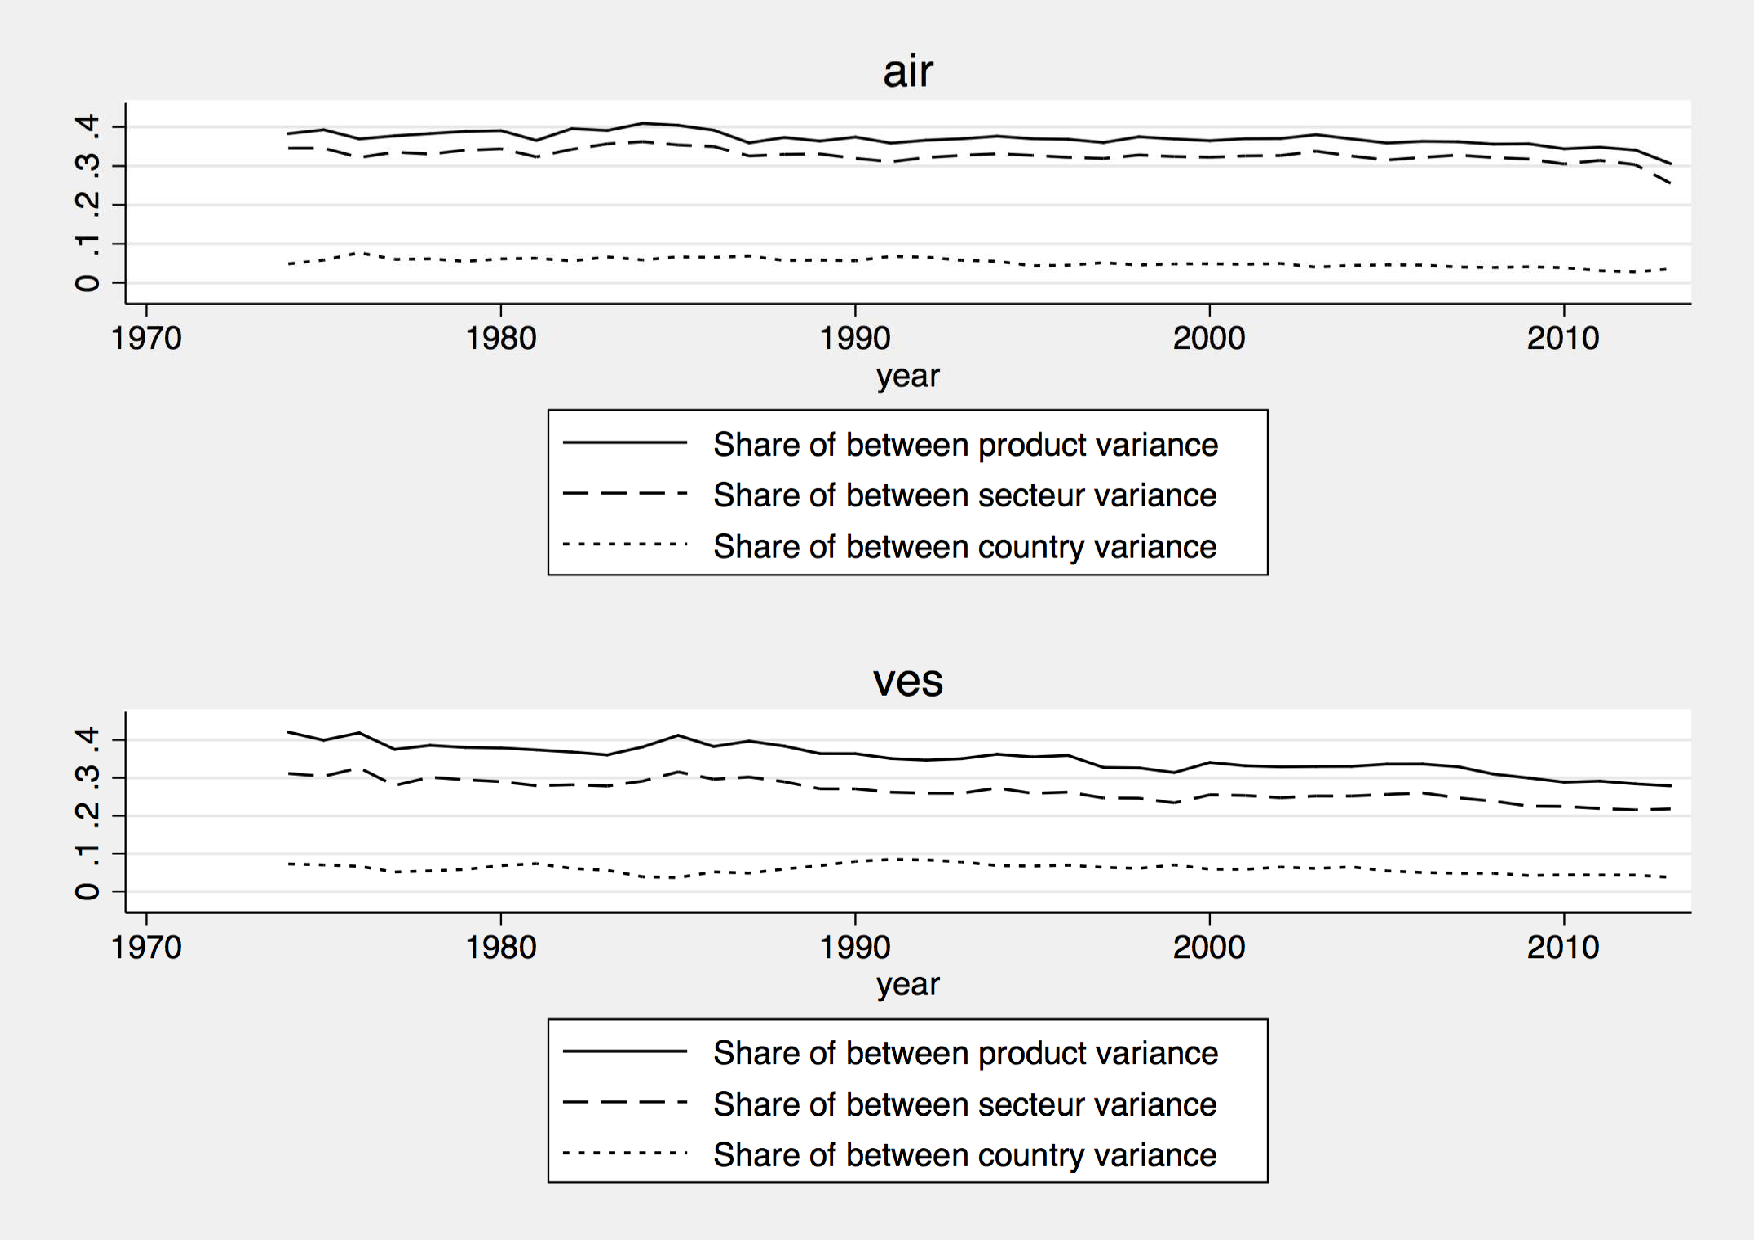
\includegraphics[width=10cm, height=7cm]{variance_decomposition.pdf}
%{\footnotesize {OECD data} }
\end{center}
\end{figure}

Two interesting results emerge from Figure \ref{fig:decomp_variance}.
First, the share of the cif-fas price gap variance that comes from the variance between products (5-digit level) is of same magnitude of order at the variance between sectors at the 3-digit level.
Both account for between 30 and 40\% of the total variance in Air transport, depending on the years considered.
This is also the case for vessel transport, even if the difference between the between-product variance share and the between-sector share is more pronounced (30\% for the between-sector vs 40\% for the between-product variance at the beginning of the period).
This delivers an indirect robustness check to the degree of classification we have retained to estimate international transport costs.
Second, the variance of the cif-fas price gap that can be attributed to the product (or sector) dimension is much larger than the between-country variance.
This holds throughout the period and for both transport modes.
This suggests that what primarily matters in international transport costs is mostly attributable to the product \textit{per se}, rather than to the country where it comes from.
%JH: un peu too much, non ? "By extension, one can expect a limited role of distance and other country-related variables as determinants of transport costs."


\clearpage
\setcounter{table}{0}
\setcounter{figure}{0}
\renewcommand{\thefigure}{C.\arabic{figure}}
\renewcommand{\thetable}{C.\arabic{table}}

\section{Estimation at the 4-digit level \label{app:4digit}}

In this section, we report the estimation results when we retain the 4-digit classification level ($s$=4-digit).

\subsection{Transport cost estimates}


Tables \ref{tab:result_air_rob} and \ref{tab:result_ves_rob} report the estimates of both models (with and without additive costs) in Air and Ocean transport respectively.

\begin{table}[htbp]
  \centering
  \caption{Air: Transport costs estimates, Selected years, 4-digit}
\begin{center}
  \footnotesize{
    \begin{tabular}{l|cccccc}
   \hline\hline
Year & 1974  & 1981  & 1989  & 2001  & 2009  & 2013 \\ \hline
\multicolumn{7}{l}{\textbf{Model (a) - With only Ad-Valorem TC} ($\widehat{\tau}^{ice}-1$, in \%) }  \\
\hline
Mean  & 6.6 & 5.8 & 5.2 & 3.3 & 3.7 & 3.2 \\
Median & 5.2 & 4.4 & 4.1 & 2.1 & 2.7 & 2.6 \\
%Standard Error & 0.056 & 0.054 & 0.046 & \multicolumn{1}{c}{0.040} & \multicolumn{1}{c}{0.036} & \multicolumn{1}{c}{0.025}  \\
\hline
\multicolumn{7}{l}{\textbf{Model (b) - With Additive \& Ad-Valorem TC}}  \\ \hline
\multicolumn{7}{l}{\textit{Ad-valorem term }($\widehat{\tau}^{adv}-1$, in \%) }   \\ \hline
Mean  & 3.5 & 2.6 & 3.1 & 1.5 & 2.1 & 1.6  \\
Median & 2.5 & 1.7 & 1.9 & 1.0 & 1.7 & 1.4  \\
%Standard Error & 0.036 & 0.028 & 0.030 & \multicolumn{1}{c}{0.021} & \multicolumn{1}{c}{0.024} & \multicolumn{1}{c}{0.015}  \\
\hline
\multicolumn{7}{l}{\textit{Additive term} ($\widehat{t}/\widetilde{p}$), in \%}    \\ \hline
Mean  & 2.6 & 2.1 & 1.7 & 1.2 &1.2 & 1.0 \\
Median & 1.2 & 0.6 & 0.6 & 0.5 & 0.4 & 0.4  \\
%Standard Error & 0.039 & 0.042 & 0.033 & \multicolumn{1}{c}{0.027} & \multicolumn{1}{c}{0.029} & \multicolumn{1}{c}{0.019} \\
\hline
\# observations & 14944 & 16844 & 25307 & \multicolumn{1}{c}{35005} & \multicolumn{1}{c}{38475} & \multicolumn{1}{c}{39460}  \\
\hline\hline
\multicolumn{7}{l}{\parbox[l]{11cm}{ \vspace{7pt}\scriptsize{Notes: TC = Transport Costs.
Statistics are obtained weighting each observation by its share in trade (mode-dependent).
Additive term expressed in fraction of fas price.}}}
\end{tabular}%
}
\end{center}
  \label{tab:result_air_rob}
\end{table}%


\begin{table}[htbp]
  \centering
\caption{Vessel: Transport costs estimates, Selected years, 4-digit}
\begin{center}
  \footnotesize{
    \begin{tabular}{l|cccccc}
   \hline\hline
Year & 1974  & 1981  & 1989  & 2001  & 2009  & 2013 \\
\hline
\multicolumn{7}{l}{\textbf{Model (a) - With only Ad-Valorem TC} ($\widehat{\tau}^{ice}-1$, in \%)} \\
\hline
Mean  & 9.8 & 6.1 & 5.8 & 5.1 & 4.2 & 3.6  \\
Median & 9.4 & 5.1 & 4.8 & 4.5 & 3.8 & 3.1 \\
%Standard Error & 0.060 & 0.038 & \multicolumn{1}{c}{0.036} & \multicolumn{1}{c}{0.030} & \multicolumn{1}{c}{0.023} & \multicolumn{1}{c}{0.020} \\
\hline
\multicolumn{7}{l}{\textbf{Model (b) - With Additive \& Ad-Valorem TC} }\\ \hline
\multicolumn{7}{l}{\textit{Ad-valorem term} ($\widehat{\tau}^{adv}-1$, in \%) }   \\ \hline
Mean  & 5.4 & 3.4 & 2.8 & 2.8 & 2.4 & 2.1  \\
Median & 4.9 & 3.0 & 2.4 & 2.5 & 2.6 & 1.8 \\
%Standard Error & 0.043 & 0.026 & \multicolumn{1}{c}{0.025} & \multicolumn{1}{c}{0.021} & \multicolumn{1}{c}{0.016} & \multicolumn{1}{c}{0.013}  \\
\hline
\multicolumn{7}{l}{\textit{Additive term} ($\widehat{t}^{add}/\widetilde{p}$, in \%) }   \\ \hline
Mean  & 4.6 & 2.6 & 3.1 & 2.4 & 2.1 & 1.5  \\
Median & 2.9 & 1.3 & 1.9 & 1.5 & 1.3 & 0.8 \\
%Standard Error & 0.068 & 0.044 & \multicolumn{1}{c}{0.037} & \multicolumn{1}{c}{0.035} & \multicolumn{1}{c}{0.031} & \multicolumn{1}{c}{0.023} \\
\hline
\# observations & 19196 & 17916 & \multicolumn{1}{c}{29387} & \multicolumn{1}{c}{36677} & \multicolumn{1}{c}{37643} & \multicolumn{1}{c}{38820} \\
\hline\hline
\multicolumn{7}{l}{\parbox[l]{11cm}{ \vspace{7pt}\scriptsize{Notes: TC = Transport Costs.
Statistics are obtained weighting each observation by its share in trade (mode-dependent).
Additive term expressed in fraction of fas price.}}}
\end{tabular}%
}
\end{center}
\label{tab:result_ves_rob}%
\end{table}%

\subsection{Goodness-of-fit tests at the 4-digit level}

We now report the goodness-of-fit exercise (conducted by transport mode) at the 4-digit product classification level (for the selected years).
The results are reported in Tables \ref{tab:good_fit_air_rob} (for Air) and \ref{tab:good_fit_ves_rob} (for Vessel).
\begin{table}[htbp]
  \centering
  \caption{Air: Measures of Goodness-of-fit, 4-digits}
\begin{center}
\label{tab:good_fit_air_rob}%
%\vspace{0.5cm}
%\scalebox{0.97}{
  \footnotesize{
\begin{tabular}{l|cccccc}
\hline
\hline
      & \multicolumn{6}{c}{Year}              \\
      & \multicolumn{1}{c}{1974} & \multicolumn{1}{c}{1981} & \multicolumn{1}{c}{1989} & \multicolumn{1}{c}{2001} & \multicolumn{1}{c}{2009} & \multicolumn{1}{c}{2013}  \\
\hline
\textbf{R2} & \multicolumn{1}{c}{} & \multicolumn{1}{c}{} & \multicolumn{1}{c}{} &       &       &      \\
Model (a)& \multicolumn{1}{c}{0.48} & \multicolumn{1}{c}{0.49} & \multicolumn{1}{c}{0.50} & \multicolumn{1}{c}{0.50} & \multicolumn{1}{c}{0.45} & \multicolumn{1}{c}{0.35} \\
Model (b) & \multicolumn{1}{c}{0.63} & \multicolumn{1}{c}{0.66} & \multicolumn{1}{c}{0.65} & \multicolumn{1}{c}{0.66} & \multicolumn{1}{c}{0.54} & \multicolumn{1}{c}{0.45} \\
\textbf{SER} & \multicolumn{1}{c}{} & \multicolumn{1}{c}{} & \multicolumn{1}{c}{} &       & \multicolumn{1}{c}{} & \multicolumn{1}{c}{}  \\
Model (a)& \multicolumn{1}{c}{0.8} & \multicolumn{1}{c}{0.9} & \multicolumn{1}{c}{0.83} &   0.87    & \multicolumn{1}{c}{0.88} & \multicolumn{1}{c}{0.93}  \\
Model (b) & \multicolumn{1}{c}{0.67} & \multicolumn{1}{c}{0.74} & \multicolumn{1}{c}{0.69} &  0.80     & \multicolumn{1}{c}{0.80} & \multicolumn{1}{c}{0.86}  \\
\textbf{Log-likelihood} & \multicolumn{1}{c}{} & \multicolumn{1}{c}{} & \multicolumn{1}{c}{} &       & \multicolumn{1}{c}{} & \multicolumn{1}{c}{} \\
Model (a) & \multicolumn{1}{c}{-17505.6} & \multicolumn{1}{c}{-21813.5} & \multicolumn{1}{c}{-30960.6} & \multicolumn{1}{c}{-44067.6} & \multicolumn{1}{c}{-49375.6} & \multicolumn{1}{c}{-53197.9}  \\
Model (b) & \multicolumn{1}{c}{-14895.8} & \multicolumn{1}{c}{-18589.9} & \multicolumn{1}{c}{-26553.5} & \multicolumn{1}{c}{-37297.9} & \multicolumn{1}{c}{-45747.6} & \multicolumn{1}{c}{-49899.1}  \\
\textbf{AIC criteria} & \multicolumn{1}{c}{} & \multicolumn{1}{c}{} & \multicolumn{1}{c}{} &       & \multicolumn{1}{c}{}  \\
Model (a)& \multicolumn{1}{c}{36243.1} & \multicolumn{1}{c}{44966.9} & \multicolumn{1}{c}{63417.1} & \multicolumn{1}{c}{89747.2} & \multicolumn{1}{c}{100317.13} & \multicolumn{1}{c}{107963.7} \\
Model (b) & \multicolumn{1}{c}{31873.6} & \multicolumn{1}{c}{39495.8} & \multicolumn{1}{c}{55777.1} & \multicolumn{1}{c}{77439.9} & \multicolumn{1}{c}{94059.1} & \multicolumn{1}{c}{102224.3}  \\
\textbf{Test LL} &       &       &       &       &       &       \\
2$\times$(ll(UR) -ll(R)) & \multicolumn{1}{c}{5219.5} & \multicolumn{1}{c}{6447.1} & \multicolumn{1}{c}{8814.1} & \multicolumn{1}{c}{13539.4} & \multicolumn{1}{c}{7256.0} & \multicolumn{1}{c}{6597.5}  \\
\# restrictions  & \multicolumn{1}{c}{640} & \multicolumn{1}{c}{698} & \multicolumn{1}{c}{778} & \multicolumn{1}{c}{833} & \multicolumn{1}{c}{824} & \multicolumn{1}{c}{818}  \\
p-value & \multicolumn{1}{c}{0.00} & \multicolumn{1}{c}{0.000} & \multicolumn{1}{c}{0.00} & \multicolumn{1}{c}{0.00} & \multicolumn{1}{c}{0.00} & \multicolumn{1}{c}{0.000} \\
\hline\hline
\multicolumn{7}{l}{\parbox[l]{13cm}{ \vspace{7pt}\scriptsize{Notes: Model (a) = with only ad-valorem transport costs.
Model (b) = with additive \& ad-valorem
transport costs.
$R^{2}$ between the log of predicted ratio and the log of the observed ratio.
The number \# of restrictions is equal to the number of parameters estimated, i.e., the number of partner countries plus the number of products.}}}
\end{tabular}%
}
\end{center}
\end{table}%


\begin{table}[htbp]
  \centering
  \caption{Vessel: Measures of Goodness-of-fit, 4-digits}
\begin{center}
\label{tab:good_fit_ves_rob}%
  \footnotesize{
\begin{tabular}{l|cccccc}
\hline
\hline
      & \multicolumn{6}{c}{Year}                   \\
      & \multicolumn{1}{c}{1974} & \multicolumn{1}{c}{1981} & \multicolumn{1}{c}{1989} & \multicolumn{1}{c}{2001} & \multicolumn{1}{c}{2009} & \multicolumn{1}{c}{2013}  \\ \hline
\boldmath{}\textbf{R$^{2}$}\unboldmath{} &       &       &       &       &       &         \\
Term I only & 0.50  & 0.45  & \multicolumn{1}{c}{0.47} & \multicolumn{1}{c}{0.41} & \multicolumn{1}{c}{0.37} & \multicolumn{1}{c}{0.35} \\
Terms A \& I & 0.66  & 0.62  & \multicolumn{1}{c}{0.62} & \multicolumn{1}{c}{0.58} & \multicolumn{1}{c}{0.51} & \multicolumn{1}{c}{0.46} \\
\textbf{SER} &       &       & \multicolumn{1}{c}{} & \multicolumn{1}{c}{} & \multicolumn{1}{c}{} & \multicolumn{1}{c}{} \\
Model (a) &    0.58   &   0.64    & \multicolumn{1}{c}{0.61} & \multicolumn{1}{c}{0.0.72} & \multicolumn{1}{c}{0.79} & \multicolumn{1}{c}{0.82} \\
Model (b) &   0.48    &    0.53   & \multicolumn{1}{c}{0.51} & \multicolumn{1}{c}{0.61} & \multicolumn{1}{c}{0.69} & \multicolumn{1}{c}{0.75} \\
\textbf{Log-likelihood} &       &       & \multicolumn{1}{c}{} & \multicolumn{1}{c}{} & \multicolumn{1}{c}{} & \multicolumn{1}{c}{} \\
Model (a)& -16460.1 & -16951.6 & \multicolumn{1}{c}{-26771.4} & \multicolumn{1}{c}{-39008.3} & \multicolumn{1}{c}{-43888.9} & \multicolumn{1}{c}{-47161.6} \\
Model (b) & -12743.65 & -13546.9 & \multicolumn{1}{c}{-21752.8} & \multicolumn{1}{c}{-33281.0} & \multicolumn{1}{c}{-39078.9} & \multicolumn{1}{c}{-43399.2}  \\
\textbf{AIC criteria} &       &       & \multicolumn{1}{c}{} & \multicolumn{1}{c}{} & \multicolumn{1}{c}{} & \multicolumn{1}{c}{} \\
Model (a) & 34464.2 & 35491.2 & \multicolumn{1}{c}{55272.9} & \multicolumn{1}{c}{79800.7} & \multicolumn{1}{c}{89459.8} & \multicolumn{1}{c}{95987.2}\\
Model (b) & 28271.3 & 29877.8 & \multicolumn{1}{c}{46595.6} & \multicolumn{1}{c}{69743.9} & \multicolumn{1}{c}{81155.7} & \multicolumn{1}{c}{89692.4} \\
\textbf{Test LL} &       &       & & &  & \\
2$\times$(ll(UR) -ll(R)) & 12385.80 & 11226.8 & \multicolumn{1}{c}{17354.7} & \multicolumn{1}{c}{20113.5} & \multicolumn{1}{c}{16608.2} & \multicolumn{1}{c}{12589.6} \\
\# restrictions  & 797   & 814   & \multicolumn{1}{c}{881} & \multicolumn{1}{c}{910} & \multicolumn{1}{c}{886} & \multicolumn{1}{c}{874} \\
p-value & 0.000 & 0.000 & \multicolumn{1}{c}{0.000} & \multicolumn{1}{c}{0.000} & \multicolumn{1}{c}{0.000} & \multicolumn{1}{c}{0.000} \\
\hline\hline
\multicolumn{7}{l}{\parbox[l]{13cm}{ \vspace{7pt}\scriptsize{Notes: Model (a) = with only ad-valorem transport costs.
Model (b) = with additive \& ad-valorem
transport costs.
$R^{2}$ between the log of predicted ratio and the log of the observed ratio.
The number \# of restrictions is equal to the number of parameters estimated, i.e., the number of partner countries plus the number of products.}}}
\end{tabular}%
}
\end{center}
\end{table}%

\newpage


\clearpage
\setcounter{table}{0}
\setcounter{figure}{0}
\renewcommand{\thefigure}{D.\arabic{figure}}
\renewcommand{\thetable}{D.\arabic{table}}

\section{Eliminating the composition effects: More details \label{app:comp-effects}}

In this section, we explain in more details the method employed to eliminate the country- and product- dimensions of the estimated transport cost.

\subsection{More on our methodology}


\subsubsection{Additive and ad-valorem transport costs: Excluding the composition effects}

In this section, we detail our methodology to extract the time trend in the pure (or fitted) transport cost component, for each the ad-valorem and the additive component.

\paragraph{For the ad-valorem component} Consider first the multiplicative transport cost component.
Rewriting Equation (\ref{eq:compeffects_mult}) by taking the exponential, we get:

\begin{equation*}
\widehat{\tau}_{ikt}=\exp\left(\delta + \sum_{i \neq \text{AFG}}\alpha_i.\mathbbm{1}_i+\sum_{k\neq \text{011}}\beta_k.\mathbbm{1}_k\right).\exp\left(\sum_{t \neq 1974}\gamma_t.\mathbbm{1}_t\right) .\exp\left(\epsilon_{ikt}\right)
\end{equation*}

Based on this equation, we deduce after estimation that:

\[\left\{
  \begin{array}{lcl}
  \text{For the year 1974:} &&  \widehat{\tau}_{is74} = \exp(\delta +\alpha_i+\beta_s), \\
  \text{For any year }t> 1974:&& \widehat{\tau}_{ist} = \exp(\delta +\alpha_i+\beta_s)\times \exp(\gamma_t) \\
  \end{array}
\right.\]

From this, we obtain the following recursive link: $\widehat{\tau}_{ist} = \widehat{\tau}_{is74}\exp(\gamma_t)$.
Given that $\tau >1$, we can rewrite to get the percentage change between year 1974 and any year $t>1974$:
\begin{equation*}
\Gamma_{ist} = 100.\frac{\widehat{\tau}_{ist}-1}{\widehat{\tau}_{is74}-1} = 100.\frac{\widehat{\tau}_{is74}\exp(\gamma_t)-1}{\widehat{\tau}_{is74}-1}
\end{equation*}

As such, the index of transport costs in year $t$ (relative to the reference year 1974) $\Gamma_{ist} $  only depends on the cost observed in 1974 and the time trend.
At this stage though, it remains specific to a product-origin country pair.
Next step is to build the index $\Gamma^{adv}_t$ such that:
\begin{equation}
 \Gamma^{adv}_t= 100\frac {\bar{\tau}_{1974}.\exp(\gamma_t)-1} {\bar{\tau}_{1974}-1}  \label{eq:tcadv_compoeffect}
\end{equation}
\noindent that is, Equation (\ref{eq:comp_effects_adv}) with $\bar{\tau}_{1974} = \exp(\delta + \sum_i \alpha_i + \sum_k \beta_k$) the mean (ad-valorem) transport cost in 1974.

\paragraph{For the additive component} After estimating Equation (\ref{eq:compeffects_add}), we can re-build the additive component according to:
\[\left\{
  \begin{array}{lcl}
\text{For the year 1974:}&&\widehat{t}_{is74}=  \delta + \alpha_i+ \beta_s, \\
\text{For any year}~t> 1974:&&\widehat{t}_{ist}=\left(\delta + \alpha_i+ \beta_s\right).\exp(\gamma_t)
\end{array}
\right.\]

From this, we deduce the recursive link: $\widehat{t}_{ist} = \widehat{t}_{is74} \times \exp(\gamma_t)$.
Given the constraint $t>0$, we then obtain the percentage change from 1974 from:

\begin{equation}
\Gamma^{add}_{ist} = 100\frac{\widehat{t}_{ist}}{\widehat{t}_{ik74}} = 100\exp(\gamma_t) \label{eq:indice_add}
\end{equation}

\noindent Note that it is independent of the product-origin country pair, we can thus rewrite the time-trend series for the additive transport cost component as:
\begin{equation}
\Gamma^{add}_t  = 100\exp(\gamma_t) \label{eq:tcadd_compoeffect}
\end{equation}


\subsection{Comparing with \cite{hummels2007} \label{app:compare_Hummels}}

In this section, we investigate the difference of results with \cite{hummels2007} regarding the importance of the composition effects in characterizing the time trends of international transport costs.
In order to do so, we start from the empirical specification implemented by \cite{hummels2007} (also making use of Hummels' Stata codes provided on his webpage\footnote{\url{http://www.krannert.purdue.edu/faculty/hummelsd/research/jep-transport-cost-data.php}}), to better identify the precise points of difference between our estimation strategies.

Let us start from Hummels' (2007) quotation (p.
146) according to which (for air), the ``\textit{unadjusted measure of ad valorem air shipping costs [is] the aggregate expenditures on air shipping divided by the value of airborne imports}''.
From this, we get the ``raw'' ad-valorem measure of transport costs as the ratio between the imported total value and the exported total value ($(p_{ikt} - \widetilde{p}_{ikt})q_{ikt}/\widetilde{p}_{ikt}q_{ikt})$, the mean yearly value being obtained by weighting each flow by its value in total trade flows (ie, yielding the observed aggregate value of $\tau_t$ for air).

Consider now the ``fitted ad-valorem rate''.
\cite{hummels2007} uses ``\textit{a regression in which the dependent variable is the ad-valorem air freight cost in logs for commodity $k$ shipped from exporter} $i$\footnote{To be consistent with our notations, we change the country subscript from $j$ (Hummels' (2007) terminology) to $i$ (our terminology).} \textit{at time $t$.
The independent variables include a separate intercept for each exporter-commodity shipped, the weight/value ratio in logs for each shipment, and year dummy variables}''.
With the value of the shipment equal to $\widetilde{p}_{ikt}q_{ikt}$, and denoting the air freight cost as $TC_{ikt}$, we can formulate the above sentence according to the following equation (suppressing the transport mode index to alleviate notation):

\begin{eqnarray}
&&\ln TC_{ikt} = \delta+ \beta \ln \frac{q_{ikt}}{\widetilde{p}_{ikt}q_{ikt}} + \sum_{i,k}\alpha_{ik}.\mathbbm{1}_{ik}+ \sum_{t}\gamma_{t}.\mathbbm{1}_{t} + \epsilon_{ikt} \notag \\
\Leftrightarrow && \ln TC_{ikt} = \delta+ \beta \ln \frac{1}{\widetilde{p}_{ikt}} + \sum_{i,k}\alpha_{ik}.\mathbbm{1}_{ik}+ \sum_{t}\gamma_{t}.\mathbbm{1}_{t} + \epsilon_{ikt} \label{eq:Hummels1}
\end{eqnarray}

\noindent where $TC_{ikt}$ is measured by the ratio between (air) charges, i.e.
$(p_{ikt} - \widetilde{p}_{ikt})q^{fas}_{ikt}$ and the value of the shipment, i.e.
$\widetilde{p}_{ikt}q^{fas}_{ikt}$, or equivalently : $TC_{ikt} = \frac{p_{ikt} - \widetilde{p}_{ikt}}{\widetilde{p}_{ikt}}$.\medskip

After estimating Equation (\ref{eq:Hummels1}), \cite{hummels2007} uses the predicted value of the regression, denoted $\widehat{TC}_{ikt}$, to obtain the unweighed average in the product/origin country dimension $i,k$, that is $\widehat{TC}_{t}$, to be compared to the unfitted ad-valorem rate $TC_{t}$ (by transport mode).\medskip

What are the main differences with our estimation strategy? Five points may be underlined.
First, \cite{hummels2007} obtains the fitted ad-valorem rate in one step (considering the observed export-import price gap on the left-hand side of Equation (\ref{eq:Hummels1})), while we use our two-step approach to extract the fitted transport cost (ie, composition effect excluded) from the (already estimated) unfitted rate.
However, this is a slight difference, as in both cases it ultimately amounts taking the predicted value of Equation (\ref{eq:Hummels1}) (which eliminates the changes specific to the origin country/product/year triplet).
Second, in contrast to us, \cite{hummels2007} does not purge its measure of the fitted ad-valorem rate by the country-sector fixed effects.
This is not likely to make a substantial difference though, as these fixed effects are by nature constant over time.
Accordingly, they only play as a scale effect as the estimate is in log.

A third difference is that we separate the country-product fixed effects ($\sum_{i,k}\alpha_{ik}.\mathbbm{1}_{ik}$ in Equation (\ref{eq:Hummels1})) in two separate components (origin country and product dimensions).
As discussed in Section \ref{sec:robustness}, this is constrained by the number of fixed effects to estimate.
However, we do not view this as the major cause of difference between our two methods, as it can be inferred from the robustness analysis on this point in Section \ref{sec:robustness}.

Fourth, we differ in the weighting scheme retained to obtain the yearly value of the fitted transport cost (in the terms of \citeh{hummels2007} method, the switch from $\widehat{TC}_{ikt}$ to $\widehat{TC}_{t}$, Equations (\ref{eq:comp_effects_adv}) and (\ref{eq:comp_effects_add}) in our case).
\cite{hummels2007} takes the unweighed average value over the $i,k$ dimension, which implicitly attributes a weight equal to 1 to each flow.
We proceed differently, as we weight each flow by its relative value on total trade flows observed in 1974.
This choice is made for two reasons.
First, this weighting scheme does not overweight the small flows in value.
Second, considering the 1974 weighting scheme makes sense as starting point of our time trend analysis.
However, we ensure that our results are not sensitive to an alternative weighting scheme, by building the average fitted transport costs rate as in \cite{hummels2007}, as reported in Section \ref{sec:robustness}.

One last difference remains to be commented, which relies on the way the additive component of international transport costs is treated.
As we show below, it turns out to be key in accounting for the difference of results with \cite{hummels2007}.
Coming back to Equation (\ref{eq:Hummels1}), it can be shown that it encompasses the two extreme cases of only ad-valorem costs ($\beta = 0$) and only additive costs ($\beta=1$), as also pointed out in \cite{hummels_skiba}.
To see it clearly, rewrite Equation (\ref{eq:Hummels1}) in a simpler form as:

$$\ln TC_{ikt} \equiv \ln \left(\frac{p_{ikt}- \widetilde{p}_{ikt}}{\widetilde{p}_{ikt}} \right) = \Delta_{ikt}- \beta \ln \widetilde{p}_{ikt} $$

\noindent with $\Delta_{ikt} \equiv \sum_{i,k}\alpha_{ik}.\mathbbm{1}_{ik}+ \sum_{t}\gamma_{t}.\mathbbm{1}_{t}$ agglomerates the various fixed effects for reading clarity.

Under the first polar case with $\beta = 1$, it becomes:
\begin{eqnarray*}
&&\ln \left(\frac{p_{ikt}- \widetilde{p}_{ikt}}{\widetilde{p}_{ikt}} \right) = \Delta_{ikt}- \ln \widetilde{p}_{ikt} \\
\Leftrightarrow && \ln (p_{ikt}- \widetilde{p}_{ikt}) = \Delta_{ikt} \\
\end{eqnarray*}
\noindent Equivalently, we can write:

\begin{eqnarray*}
&&p_{ikt} = \widetilde{p}_{ikt} + \exp(\Delta_{ikt})\\
\Leftrightarrow && p_{ikt} = \widetilde{p}_{ikt} + t_{ikt}
\end{eqnarray*}
\noindent with $t_{ikt}$ appropriately defined.
This exactly corresponds to the case of additive costs only.

In the second polar case with $\beta = 0$, Equation (\ref{eq:Hummels1}) becomes:
\begin{eqnarray*}
&&\ln \left(\frac{p_{ikt}- \widetilde{p}_{ikt}}{\widetilde{p}_{ikt}} \right) = \Delta_{ikt} \\
\Leftrightarrow && \ln \left(\frac{p_{ikt}}{\widetilde{p}_{ikt}}-1\right) = \Delta_{ikt}\\
\Leftrightarrow && \frac{p_{ikt}}{\widetilde{p}_{ikt}}  = \exp (\Delta_{ikt})+1
\end{eqnarray*}
\noindent that is,

$$p_{ikt} = \tau_{ikt} \widetilde{p}_{ikt}$$

\noindent with $\tau_{ikt}$ appropriately defined.
This exactly corresponds to the case of ad-valorem transport costs only.


As noted by \cite{hummels_skiba}, $0<\beta<1$ represents the elasticity of freight costs to the export prices, increasing with the relative weight of the additive component in international transport costs.
By estimating Equation (\ref{eq:Hummels1}) with a constant $\beta$, \cite{hummels2007} assumes that the share of additive costs does not vary over time, country partner or product.
This is an important difference with our method, as we measure transport costs by explicitly allowing for an additive component that varies in the three dimensions (ie, somehow allowing for a varying $\beta$ across time, country partner and product).
To establish this point clearly, we replicate the method adopted by \cite{hummels2007} exposed above on our database (which is the same as his until 2004).
The results are reported in Figure \ref{fig:comp_effects_as_in_Hummels}.






\end{document}

